%TODO alles zusammenfügen und in ein Dokument mit REPORT und Chapters (gemäss Ordnerstruktur)
\documentclass[11pt,a4paper, parskip,ngerman] {report} 


%Preamble for the Document for reuse and the last Document
\author{\authors}
\date{\today{}}
\title{\arbeit}
\usepackage[T1]{fontenc} % Font family encoding: 8 Bit
\usepackage[utf8]{inputenc} % Encoding in the created document: UTF-8
\usepackage[sfdefault]{FiraSans} % Font family
\renewcommand*\oldstylenums[1]{{\firaoldstyle #1}}
\usepackage[babel]{microtype} % Automatische Grauwertverbesserung
\usepackage[ngerman]{babel}
\usepackage[automark]{scrpage2}
\usepackage[colorlinks = true,
linkcolor = black]{hyperref}
\usepackage{color}
\usepackage[normalem]{ulem}
\usepackage{scrpage2}
\usepackage{graphicx}
\usepackage{tabularx}
\usepackage{textcomp}

\usepackage{framed}
\usepackage{geometry}
\usepackage{minutes}
\usepackage{lscape}
\usepackage[table]{xcolor}
\usepackage{multicol}
\usepackage{longtable,tabu}

\usepackage[style=numeric,,sorting=none,backend=bibtex]{biblatex}
\addbibresource{./SDDC.bib}
\usepackage{titlesec}
\usepackage[printonlyused] {acronym}
\titleformat{\chapter}{\normalfont\huge\bf}{\thechapter}{20pt}{\huge\bf}
\pagestyle{plain}
\usepackage{caption}
\usepackage{subcaption}
\usepackage{pdfpages}

\usepackage{tikz}
\usepackage{pgf-pie}
\usetikzlibrary{positioning,shadings}
\usetikzlibrary{arrows}
\usepackage{pbox}
\definecolor{logocolor}{RGB}{6,103,236}
%Code Listing 
\usepackage{color}
\usepackage{listings}

\definecolor{mygreen}{rgb}{0,0.6,0}
\definecolor{mygray}{rgb}{0.5,0.5,0.5}
\definecolor{mymauve}{rgb}{0.58,0,0.82}
%Standard
\lstset{ %
  backgroundcolor=\color{white},  
  basicstyle=\footnotesize,        
  breakatwhitespace=false,         
  breaklines=true,               
  captionpos=b,                  
  commentstyle=\color{mygreen},    
  deletekeywords={...},            
  escapeinside={\%*}{*)},          
  extendedchars=true,           
  frame=single,	                   
  keepspaces=true,                 
  keywordstyle=\color{blue},      
  language=Octave,                 
  otherkeywords={*,...},           
  numbers=none,                    
  rulecolor=\color{black},         
  showspaces=false,               
  showstringspaces=false,          
  showtabs=false,                
  stepnumber=2,                    
  stringstyle=\color{mymauve},     
  tabsize=2,	                   
  title=\lstname             
}

%Java
\definecolor{dkgreen}{rgb}{0,0.6,0}
\definecolor{gray}{rgb}{0.5,0.5,0.5}
\definecolor{mauve}{rgb}{0.58,0,0.82}
\definecolor{light-gray}{gray}{0.25}

\lstdefinestyle{java}{
  language=Java,
  aboveskip=3mm,
  belowskip=3mm,
  showstringspaces=false,
  columns=flexible,
  basicstyle={\footnotesize\ttfamily},
  numberstyle={\tiny},
  numbers=none,
  keywordstyle=\color{blue},
  commentstyle=\color{dkgreen},
  stringstyle=\color{mauve},
  breaklines=true,
  breakatwhitespace=true,
  tabsize=3
}



%JSON Styles
\colorlet{punct}{red!60!black}
\definecolor{background}{HTML}{EEEEEE}
\definecolor{delim}{RGB}{20,105,176}
\colorlet{numb}{magenta!60!black}

\lstdefinelanguage{json}{
    stepnumber=1,
    breaklines=true,
    literate=
     *{0}{{{\color{numb}0}}}{1}
      {1}{{{\color{numb}1}}}{1}
      {2}{{{\color{numb}2}}}{1}
      {3}{{{\color{numb}3}}}{1}
      {4}{{{\color{numb}4}}}{1}
      {5}{{{\color{numb}5}}}{1}
      {6}{{{\color{numb}6}}}{1}
      {7}{{{\color{numb}7}}}{1}
      {8}{{{\color{numb}8}}}{1}
      {9}{{{\color{numb}9}}}{1}
      {:}{{{\color{punct}{:}}}}{1}
      {,}{{{\color{punct}{,}}}}{1}
      {\{}{{{\color{delim}{\{}}}}{1}
      {\}}{{{\color{delim}{\}}}}}{1}
      {[}{{{\color{delim}{[}}}}{1}
      {]}{{{\color{delim}{]}}}}{1},
}

%XML
\definecolor{forestgreen}{RGB}{34,139,34}
\definecolor{orangered}{RGB}{239,134,64}
\definecolor{darkblue}{rgb}{0.0,0.0,0.6}
\definecolor{gray}{rgb}{0.4,0.4,0.4}

\lstdefinestyle{XML} {
    language=XML,
    extendedchars=true, 
    breaklines=true,
    breakatwhitespace=true,
    emph={},
    emphstyle=\color{red},
    basicstyle=\ttfamily,
    columns=fullflexible,
    commentstyle=\color{gray}\upshape,
    morestring=[b]",
    morecomment=[s]{<?}{?>},
    morecomment=[s][\color{forestgreen}]{<!--}{-->},
    keywordstyle=\color{orangered},
    stringstyle=\ttfamily\color{black}\normalfont,
    tagstyle=\color{darkblue}\bf,
    morekeywords={attribute,xmlns,version,type,release},
    otherkeywords={attribute=, xmlns=},
}


%Bash
\lstdefinestyle{Bash}
{
 language=bash,
 frame=single,
  showstringspaces=false,
  commentstyle=\color{green},
  keywordstyle=\color{blue}
}

\titlespacing*{\subsection}
{0pt}{5.5ex plus 1ex minus .2ex}{4.3ex plus .2ex}

\usepackage{glossaries}
\makeglossaries
%Definition of frequently used Texts
\newcommand{\advisor}
	{Urs Baumann}
\newcommand{\advisorprof}
	{Prof. Beat Stettler}
\newcommand{\contraprof}
	{TBA}
\newcommand{\expert}
	{TBA}
\newcommand{\authors}
	{Silvan Adrian, Fabian Binna}
\newcommand{\place}
	{Hochschule für Technik Rapperswil \\ Institute for Networked Solutions}
\newcommand{\ins}
	{Institute for Networked Solutions}
\newcommand{\timeperiod}
	{Herbstsemester 2015}
\newcommand{\titel}
	{SDDC \\ Software Defined Data Center}
\newcommand{\arbeit}
	{Semesterarbeit }	


\begin{document}
%Inputs Config
%%Definition of frequently used Texts
\newcommand{\advisor}
	{Urs Baumann}
\newcommand{\advisorprof}
	{Prof. Beat Stettler}
\newcommand{\contraprof}
	{TBA}
\newcommand{\expert}
	{TBA}
\newcommand{\authors}
	{Silvan Adrian, Fabian Binna}
\newcommand{\place}
	{Hochschule für Technik Rapperswil \\ Institute for Networked Solutions}
\newcommand{\ins}
	{Institute for Networked Solutions}
\newcommand{\timeperiod}
	{Herbstsemester 2015}
\newcommand{\titel}
	{SDDC \\ Software Defined Data Center}
\newcommand{\arbeit}
	{Semesterarbeit }	

%\documentclass[11pt,a4paper, parskip,ngerman] {report} 


%Preamble for the Document for reuse and the last Document
\author{\authors}
\date{\today{}}
\title{\arbeit}
\usepackage[T1]{fontenc} % Font family encoding: 8 Bit
\usepackage[utf8]{inputenc} % Encoding in the created document: UTF-8
\usepackage[sfdefault]{FiraSans} % Font family
\renewcommand*\oldstylenums[1]{{\firaoldstyle #1}}
\usepackage[babel]{microtype} % Automatische Grauwertverbesserung
\usepackage[ngerman]{babel}
\usepackage[automark]{scrpage2}
\usepackage[colorlinks = true,
linkcolor = black]{hyperref}
\usepackage{color}
\usepackage[normalem]{ulem}
\usepackage{scrpage2}
\usepackage{graphicx}
\usepackage{tabularx}
\usepackage{textcomp}

\usepackage{framed}
\usepackage{geometry}
\usepackage{minutes}
\usepackage{lscape}
\usepackage[table]{xcolor}
\usepackage{multicol}
\usepackage{longtable,tabu}

\usepackage[style=numeric,,sorting=none,backend=bibtex]{biblatex}
\addbibresource{./SDDC.bib}
\usepackage{titlesec}
\usepackage[printonlyused] {acronym}
\titleformat{\chapter}{\normalfont\huge\bf}{\thechapter}{20pt}{\huge\bf}
\pagestyle{plain}
\usepackage{caption}
\usepackage{subcaption}
\usepackage{pdfpages}

\usepackage{tikz}
\usepackage{pgf-pie}
\usetikzlibrary{positioning,shadings}
\usetikzlibrary{arrows}
\usepackage{pbox}
\definecolor{logocolor}{RGB}{6,103,236}
%Code Listing 
\usepackage{color}
\usepackage{listings}

\definecolor{mygreen}{rgb}{0,0.6,0}
\definecolor{mygray}{rgb}{0.5,0.5,0.5}
\definecolor{mymauve}{rgb}{0.58,0,0.82}
%Standard
\lstset{ %
  backgroundcolor=\color{white},  
  basicstyle=\footnotesize,        
  breakatwhitespace=false,         
  breaklines=true,               
  captionpos=b,                  
  commentstyle=\color{mygreen},    
  deletekeywords={...},            
  escapeinside={\%*}{*)},          
  extendedchars=true,           
  frame=single,	                   
  keepspaces=true,                 
  keywordstyle=\color{blue},      
  language=Octave,                 
  otherkeywords={*,...},           
  numbers=none,                    
  rulecolor=\color{black},         
  showspaces=false,               
  showstringspaces=false,          
  showtabs=false,                
  stepnumber=2,                    
  stringstyle=\color{mymauve},     
  tabsize=2,	                   
  title=\lstname             
}

%Java
\definecolor{dkgreen}{rgb}{0,0.6,0}
\definecolor{gray}{rgb}{0.5,0.5,0.5}
\definecolor{mauve}{rgb}{0.58,0,0.82}
\definecolor{light-gray}{gray}{0.25}

\lstdefinestyle{java}{
  language=Java,
  aboveskip=3mm,
  belowskip=3mm,
  showstringspaces=false,
  columns=flexible,
  basicstyle={\footnotesize\ttfamily},
  numberstyle={\tiny},
  numbers=none,
  keywordstyle=\color{blue},
  commentstyle=\color{dkgreen},
  stringstyle=\color{mauve},
  breaklines=true,
  breakatwhitespace=true,
  tabsize=3
}



%JSON Styles
\colorlet{punct}{red!60!black}
\definecolor{background}{HTML}{EEEEEE}
\definecolor{delim}{RGB}{20,105,176}
\colorlet{numb}{magenta!60!black}

\lstdefinelanguage{json}{
    stepnumber=1,
    breaklines=true,
    literate=
     *{0}{{{\color{numb}0}}}{1}
      {1}{{{\color{numb}1}}}{1}
      {2}{{{\color{numb}2}}}{1}
      {3}{{{\color{numb}3}}}{1}
      {4}{{{\color{numb}4}}}{1}
      {5}{{{\color{numb}5}}}{1}
      {6}{{{\color{numb}6}}}{1}
      {7}{{{\color{numb}7}}}{1}
      {8}{{{\color{numb}8}}}{1}
      {9}{{{\color{numb}9}}}{1}
      {:}{{{\color{punct}{:}}}}{1}
      {,}{{{\color{punct}{,}}}}{1}
      {\{}{{{\color{delim}{\{}}}}{1}
      {\}}{{{\color{delim}{\}}}}}{1}
      {[}{{{\color{delim}{[}}}}{1}
      {]}{{{\color{delim}{]}}}}{1},
}

%XML
\definecolor{forestgreen}{RGB}{34,139,34}
\definecolor{orangered}{RGB}{239,134,64}
\definecolor{darkblue}{rgb}{0.0,0.0,0.6}
\definecolor{gray}{rgb}{0.4,0.4,0.4}

\lstdefinestyle{XML} {
    language=XML,
    extendedchars=true, 
    breaklines=true,
    breakatwhitespace=true,
    emph={},
    emphstyle=\color{red},
    basicstyle=\ttfamily,
    columns=fullflexible,
    commentstyle=\color{gray}\upshape,
    morestring=[b]",
    morecomment=[s]{<?}{?>},
    morecomment=[s][\color{forestgreen}]{<!--}{-->},
    keywordstyle=\color{orangered},
    stringstyle=\ttfamily\color{black}\normalfont,
    tagstyle=\color{darkblue}\bf,
    morekeywords={attribute,xmlns,version,type,release},
    otherkeywords={attribute=, xmlns=},
}


%Bash
\lstdefinestyle{Bash}
{
 language=bash,
 frame=single,
  showstringspaces=false,
  commentstyle=\color{green},
  keywordstyle=\color{blue}
}

\titlespacing*{\subsection}
{0pt}{5.5ex plus 1ex minus .2ex}{4.3ex plus .2ex}

\usepackage{glossaries}
\makeglossaries


%\begin{document}
\newgeometry{left=2.25cm, right=2.25cm, top=2.25cm, bottom=2.25cm} % new
% margins



\begin{titlepage}
%TODO: set logo position exactly.
\begin{center}
\begin{minipage}[t]{0.45\textwidth}
    
\includegraphics[width=\textwidth]{./22_Grafiken/01_Logo/hsrLogo}
\end{minipage}
\hspace{\fill} % horizontal space
\begin{minipage}[t]{0.45\textwidth}
    \vspace{-2.9cm}
    
\includegraphics[width=\textwidth]{./22_Grafiken/01_Logo/ins} %TODO: more highres logo
\end{minipage}

\end{center}

\vspace{15ex} % vertical space
\begin{center}
	\Huge 
	\begin{framed}
		\textbf{\titel}
	\end{framed}
	
	\vspace{3ex}
	\textbf{\arbeit}
	
	\vspace{1ex}
	\LARGE 
	\place
	
	\vspace{5ex}
	\begin{framed}
		\timeperiod
	\end{framed}
\end{center}

\vspace{11ex}
\begin{tabular}{ll} % Table
	Autoren:         		& \authors	\\
	Betreuender Dozent:		& \advisorprof  	\\
	Betreuer:        		& \advisor    	\\
	Gegenleser:      		& \contraprof  	\\
	Experte:      			& \expert  		\\
	Projektpartner:      	& \ins  		\\
\end{tabular}

\end{titlepage}

\restoregeometry % reset page margins
%\end{document}
\chapter*{Abstract}\addcontentsline{toc}{chapter}{Abstract}

Unter „Software Defined“ versteht man die Zentralisierung der Intelligenz in Kontrollern. Gerade moderne Data Center werden immer häufiger von Software Kontrollern gesteuert, damit die Dynamik der Bereitstellung von neuen Services massiv erhöht werden kann. Ziel ist, die Ressourcen Storage, Network und Compute abstrahiert als skalierbare Pools der „Service Ebene“ zur Verfügung zu stellen.\\
Eine RESTful API, die den Umgang mit Services, die wiederum Pakete von Ressourcen darstellen, sorgt für einen zentralen Punkt, an den diverse Systeme und Business Applikationen anknüpfen können. Damit die breite Auswahl von Libraries und Produkten in einem Data Center angesprochen werden kann, verwaltet eine generische API die Kontroller und ermöglicht den abstrakten Umgang mit Ressourcen. Die beiden abstrakten Ebenen, RESTful API und generische API, werden mit einem Workflow verbunden. Der Workflow kümmert sich um den zeitlich korrekten Ablauf der Instantiierung. Die Software kann als Webservice in einem Docker Container ausgerollt werden und benötigt danach nur noch eine Konfiguration der generischen API und der Kontroller.

\chapter*{Erklärung der Eigenständigkeit}

Ich erkläre hiermit,

\begin{itemize}
  \item dass ich die vorliegende Arbeit selber und ohne fremde Hilfe durchgeführt habe, ausser derjenigen, 
  welche explizit in der Aufgabenstellung erwähnt ist oder mit dem Betreuer schriftlich vereinbart wurde,
  \item dass ich sämtliche verwendeten Quellen erwähnt und gemäss gängigen 
  wissenschaftlichen Zitierregeln korrekt angegeben habe.
  \item das ich keine durch Copyright geschützten Materialien (z.B. Bilder) 
  in dieser Arbeit in unerlaubter Weise genutzt habe. 
\end{itemize}

\textbf{Ort, Datum:}

Raperswil-Jona, \today


\textbf{Name, Unterschrift}



\includegraphics[width=0.25\textwidth]{01_Einleitung/images/unterschrift-sadrian}

Silvan Adrian

\newpage
Ich erkläre hiermit,

\begin{itemize}
  \item dass ich die vorliegende Arbeit selber und ohne fremde Hilfe durchgeführt habe, ausser derjenigen, 
  welche explizit in der Aufgabenstellung erwähnt ist oder mit dem Betreuer schriftlich vereinbart wurde,
  \item dass ich sämtliche verwendeten Quellen erwähnt und gemäss gängigen 
  wissenschaftlichen Zitierregeln korrekt angegeben habe.
  \item das ich keine durch Copyright geschützten Materialien (z.B. Bilder) 
  in dieser Arbeit in unerlaubter Weise genutzt habe. 
\end{itemize}

\textbf{Ort, Datum:}

Raperswil-Jona, \today


\textbf{Name, Unterschrift}



Fabian Binna
\tableofcontents


\chapter{Aufgabenstellung}

Unter ``Software Defined'' versteht man die Zentralisierung der Intelligenz in Kontrollern. 
Gerade moderne Data Center werden immer mehr von Software Kontrollern gesteuert, 
damit die Dynamik der Bereitstellung von neuen Services massiv erhöht werden kann. 
So gibt es bereits Kontroller für Storage, Netzwerk und Compute Ressourcen. 
\\ \\
Ziel ist es, die Ressourcen Storage, Network und Compute abstrahiert als skalierbare Pools der 
``Service Ebene'' zu Verfügung zu stellen. Alle modernen Kontroller können über API's 
angesprochen werden, allerdings unterscheiden sich hier die verschiedenen Hersteller zum Teil stark.
\\ \\
Ziel dieser Arbeit ist die Entwicklung einer generischen Middleware/API, um verschiedene Kontroller 
möglichst einfach in Business Applikationen zu integrieren. Nach der Definition einer systemunabhängigen 
Schnittstelle sollen die verschiedenen Kontroller danach als Treiber an die API angehängt werden können. 
Zur Demonstrationszwecken soll eine rudimentäre, ca. 3 Seitige Webpage erstellt werden, welche die erstelle 
API benützt. Dabei soll je mind. ein Storage, Compute und Network Kontroller eingebunden werden.


%Analyse
\part{Technischer Bericht}



\subsection{API}
\begin{itemize}
\item Die API sollte auf einem möglichst stabilen Stand sein.
\item Es müssen die wichtigsten Provider zur Verfügung stehen.
\item Die API muss gut dokumentiert sein.
\item Es sollen verschiedene Services angesprochen werden können (Compute, Storage, Network...).
\item Keine grosse Einarbeitung, das heisst die Programmiersprache sollte nicht komplett neu sein.
\end{itemize}

Zudem sind alle Eingenschaften die das Implementieren der Software erleichtern ein 
Pluspunkt. Von Vorteil währen zusätzliche Funktionen wie z.B SSL oder Pricing. 

\subsection{User-Dashboard}
Das User-Dashboard soll eine Möglichkeit für Benutzer bieten, um einzelne Services 
abonnieren zu können.
Dabei soll sowohl \ac{IaaS}, \ac{PaaS} oder \ac{SaaS} abonniert werden können und eine Auswahl 
bieten unter vielen verschiedenen Cloud Anbietern wählen zu können (so generisch wie 
möglich).
Dabei soll der User zwischen einzelnen Angeboten der Anbieter spezifischen 
Services zu wählen bspw.: bei Google Cloud: Cloud DNS, Firewall, Netzwerke etc.
Es kann daher auch sein das nicht alle Anbieter die gleichen Services bieten und 
daher eine Auswahl gegeben werden muss, damit der Benutzer selbst entscheiden 
kann welchen Service er haben will.

\subsubsection{SDDC}
Unser Projekt soll deshalb eine einiges generische Möglichkeit bieten, um 
Service abonnieren zu können und wenn möglich so gut wie alle Cloud Anbieter zu 
unterstützen.
Dies soll möglich werden indem ein Dashboard eine generische API anspricht und 
die API alle Schritte durchführt, die nötig sind für die Erstellung des 
Services.

\subsection{Admin-Dashboard}
Dem Admin soll eine Möglichkeit geboten werden um die Software administrieren zu 
können, z.B.: Benutzerverwaltung oder etwas in der Art.

%Alle Referenzen ins Bib File verschieben
\subsection{Referenzen}
\href{https://libcloud.apache.org}{Libcloud}\\
\href{https://jclouds.apache.org}{jClouds}\\
\href{https://github.com/esl/elibcloud}{elibcloud}\\
\href{https://github.com/fog/fog/blob/master/lib/fog/openstack/docs/getting_started.md}{fog}\\
\href{https://github.com/pkgcloud/pkgcloud}{pkgcloud}\\
\href{http://http://libvirt.org/}{libvirt}\\

\newpage

\section{API Analyse}
\subsection{\href{https://libcloud.apache.org}{Libcloud}}
\textbf{Sprache: }Python\\
\textbf{Wichtigste Provider: }Rackspace, Amazon web services, CloudStack, OpenStack, DigitalOcean, Eucalyptus, Joyent, Linode, exoscale,NephoScale, Google Cloud Platform, Zerigo, CloudSigma, iKoula, libvirt\\

\subsection{\href{https://jclouds.apache.org}{jClouds}}
\textbf{Sprache: }Java\\
\textbf{Wichtigste Provider: }OpenStack, Docker, DigitalOcean, Google Cloud Platform, 
Rackspace, HP Cloud, CloudStack, Amazon web services, abiquo, CloudSigma, joyent\\

\subsection{\href{https://github.com/esl/elibcloud}{elibcloud}}
\textbf{Sprache: }Erlang\\
elibcloud ist ein Wrapper für libcloud.\\

\subsection{\href{https://github.com/fog/fog/blob/master/lib/fog/openstack/docs/getting_started.md}{fog}}
\textbf{Sprache: }Ruby\\
\textbf{Wichtigste Provider: }CloudSigma, CloudStack, GoGrid, Google Cloud Platform, Joyent, 
Libvirt, Linode, OpenStack, OpenVZ, Rackspace, Zerigo, IBM, HP\\

\subsection{\href{https://github.com/pkgcloud/pkgcloud}{pkgcloud}}
\textbf{Sprache: }JavaScript (Node.js)\\
\textbf{Wichtigste Provider: }Amazon, Azure, DigitalOcean, Joyent, OpenStack, Rackspace, Google, HP\\

\subsection{\href{http://http://libvirt.org/}{libvirt}}
\textbf{Sprache: }C\\
\textbf{Wichtigste Provider: }Xen, KVM, OpenVZ, VMware ESX, VirtualBox, IBM PowerVM\\

\newpage

\section{Support}
\subsection{Compute}
Die grösste Auswahl an Providern liefert Libcloud.JClouds hingegen 
unterstützt auch Docker, was ein grosser Vorteil gegenüber Libcloud ist. Im 
Dokument Compute.ods im Ordner 02\_Analyse\//01\_API wird genau aufgeführt, 
welche Provider von welchen APIs unterstützt werden. Es werden nur public Clouds berücksichtigt.
Für den private Cloud Bereich bietet sich hier eher Libvirt an, da neben XEN, 
KVM, Qemu und weitere unterstützt werden.

\subsection{Storage (Object/Blob)}
\textbf{libcloud}
\begin{itemize}
\item PCextreme AuroraObjects
\item Microsoft Azure (blobs)
\item CloudFiles
\item Google Storage
\item KTUCloud Storage
\item Numbus.io
\item Ninefold
\item OpenStack Swift
\item Amazon
\end{itemize}

\textbf{jclouds (BlobStore)}
\begin{itemize}
\item AWS
\item HP Helion
\item Azure
\item Rackspace
\end{itemize}

\textbf{fog}
\begin{itemize}
\item S3
\item CloudFiles
\item Google Storage
\end{itemize}

\textbf{pkgcloud}
\begin{itemize}
\item Amazon
\item Azure
\item Google
\item HP
\item OpenStack
\item Rackspace
\end{itemize}

\textbf{libvirt}
\begin{itemize}
  \item GlusterFS
  \item Sheepdog
  \item SCSI
  \item iSCSI
  \item FiberChannel
  \item NFS
  \item lvm
  \item filesystems
\end{itemize}

\subsection{Network}
Libvirt allein bietet hier mit Abstand die beste Unterstützung von Network Konfigurationen 
(VLANs, Bridges, etc.) und ist sehr auf Private Clouds ausgelegt.\\


\subsection{Other}
\subsubsection{Database}
\textbf{pkgcloud}
\begin{itemize}
\item IrisCouch
\item MongoLab
\item Rackspace
\item MongoHQ
\item RedisToGo
\end{itemize}

\subsubsection{DNS}
\textbf{libcloud}
\begin{itemize}
\item AuroraDNS
\item DigitalOcean
\item Gandi
\item Google
\item Host Virtual
\item Linode
\item Rackspace
\item AWS Route53
\item Softlayer
\item Zerigo
\end{itemize}

\textbf{fog}
\begin{itemize}
\item AWS Route53
\item Blue Box
\item DNSimple
\item Linode
\item Rackspace
\item Rage4
\item Slicehost
\item Zerigo
\end{itemize}

\textbf{pkgcloud}
\begin{itemize}
\item Rackspace
\end{itemize}

\subsubsection{Load Balancer}
\textbf{libcloud}
\begin{itemize}
\item Brightbox
\item CloudStack
\item DimensionData
\item Amazon
\item Google
\item GoGrid
\item Ninefold
\item Rackspace
\item Softlayer
\end{itemize}

\textbf{jclouds}
\begin{itemize}
\item AWS Elastic LoadBalancer
\item Rackspace
\end{itemize}

\textbf{pkgcloud}
\begin{itemize}
\item Rackspace
\end{itemize}

\subsubsection{Orchestration}
\textbf{pkgcloud (beta)}
\begin{itemize}
\item OpenStack
\item Rackspace
\end{itemize}

\subsubsection{CDN}
\textbf{fog}
\begin{itemize}
\item CloudFront
\end{itemize}

\newpage

\section{Fazit}

Im Gesamtbild schneidet libcloud am besten ab. Es bietet deutlich am meisten Compute und 
Storage Provider. Die Dokumentation ist sehr ausführlich, mit konkreten Ratschlägen zur 
Implementation (z.B. Thread Safe). Zusätzlich bietet libcloud Module für SSL und Pricing.
Jclouds ist eine Library für Java, was für uns am besten ist, da wir am meisten Erfahrung mit 
Java haben. Es gibt jedoch nicht viele Compute Provider, dafür unterstützt jclouds als einziger Docker.
Der einzige Vorteil von fog ist die Möglichkeit CDNs als Service anzubieten.
Pkgcloud unterstützt eine breite Auswahl von Services (z.B. Database, Load Balancer, DNS).
Elibcloud ist ein erlang Wrapper für libcloud und unterstützt somit das gleiche wie libcloud 
(sonlange die Version auf dem neusten stand ist). Erlang würde sich für eine parallele Umgebung eignen, 
es sind jedoch keinerlei Erlang Kenntnisse im Team vorhanden.\\
Libvirt ist allerdings die einzige API, die sich völlig auf Private Anbieter 
zugeschnitten ist (wird auch von OpenStack verwendet), wäre also die Beste 
Lösung, wenn es darum geht eine Private Cloud aufzubauen.

\textbf{Wir entscheiden uns für libvirt. Die Gründe dafür sind unten im API Matrixvergleich aufgeführt}


\subsection{libcloud}
\begin{Argumentation}
\pro Grösste Auswahl an Compute und Storage Provider.
\pro Am besten dokumentiert. Für jede Methode existiert eine Tabelle, die zeigt welche Provider damit angesprochen werden können.
\pro Ist zwar nicht Thread-Safe. Es werden jedoch konkrete Lösungsvorschläge gemacht.
\pro SSL und Pricing Module vorhanden.

\contra Team hat wenig Erfahrung mit komplexen/grossen Python Projekten.
\end{Argumentation}

\subsection{jclouds}
\begin{Argumentation}
\pro Unterstützt Docker.
\pro Java Library. Das Team hat am meisten Erfahrung mit Java.
\pro Code Examples für fast jeden Provider.

\contra Kleine Auswahl an Compute Providern.
\end{Argumentation}

\subsection{fog}
\begin{Argumentation}
\pro Es ist möglich ein CDN als Service anzubieten.

\contra Mässige Dokumentation. Es existieren zwar 
Examples, die sind aber nicht besonders aussagekräftig.
\contra Kleine Auswahl an Compute Providern.
\end{Argumentation}

\subsection{pkgcloud}
\begin{Argumentation}
\pro Grösste Auswahl an Services.
\pro Database as a Service
\pro Orchestration
\pro Explizite Unterstützung von Network.

\contra Mässige Dokumentation. Es existieren zwar Examples, die sind aber nicht besonders aussagekräftig.
\contra Kleine Auswahl an Compute Providern.
\end{Argumentation}

\subsection{libvirt}
\begin{Argumentation}
\pro Grösste Auswahl an ``Private Cloud Anbietern''.
\pro Grosse Storage Unterstützung.
\pro Explizite Unterstützung von Network.
\pro Bietet Java Library (language Bindings)

\contra Ungenügende Dokumentation. Es existieren zwar Examples und 
sonst existiert nur eine Javadoc zur Library.
\end{Argumentation}










\newgeometry{left=1cm,bottom=2cm,top=2cm,right=1cm}

\begin{landscape}
  \subsection{API Vergleichsmatrix}
  \label{API Vergleichsmatrix}
\begin{table}[h]  
  \begin{tabularx}{\linewidth}{|l|X|X|l|X|l|X|}
    \hline
    %empty
    &
    \textbf{Entwicklungsstand}
    &
    \textbf{Provider}
    &
    \textbf{Doku}
    &
    \textbf{Serviceauswahl}
    &
    \textbf{Sprache}
    &
    \textbf{Zusatz Features}
   \\
  \hline
  %begin libcloud
  \textbf{libcloud} & \cellcolor{green!25} \textbf{v0.18.0:} 
  Die API ist stabil und wird von namhaften Firmen verwendet.
  & 
  \cellcolor{green!25}
  *~35 Unterstützt die wichtigsten Provider
  & 
   \cellcolor{green!25}
   gut
  & 
   \cellcolor{green!25}
  Wenige Services, dafür umfangreiche Funktionen
  & 
     \cellcolor{yellow!25}
  Python
  & 
  \cellcolor{green!25}
  SSL, Pricing, Übertragen von Files, Ausführen von Scripts, Unit Testability, Mocks
  \\
  \hline
  %end libcloud
  %begin jclouds
 \textbf{jclouds}
& 
\cellcolor{green!25} 
\textbf{v1.9.1:} Die API ist stabil und wird von namhaften 
Firmen verwendet.
&	
\cellcolor{green!25}
*~15
Unterstützt die wichtigsten Provider und als einziger Docker
&
\cellcolor{yellow!25}
genügend
&
\cellcolor{green!25}
Wenige Services, dafür umfangreiche Funktionen	
&
\cellcolor{green!25}
Java	
&
\cellcolor{green!25}
Thread-Safe, Unit Testability, Dateiübertragung, Scriptausführung
 \\
 \hline
 %end jclouds
 \textbf{fog}
 &
 \cellcolor{yellow!25}	
 \textbf{v1.34.0:} 
 Die API ist stabil, wird jedoch von keinen namhaften Firmen verwendet
 &
 \cellcolor{red!50}
 sehr kleine Auswahl
 &
  \cellcolor{red!50}	
ungenügend	
&
 \cellcolor{red!50}
Wenige Services. Unterstützt als einziger CDNs.	
&
 \cellcolor{red!50}
Ruby
&
 \cellcolor{red!50}
\\
\hline
%end fog
%begin pkgcloud
\textbf{pkgcloud}
&
 \cellcolor{yellow!25}	
\textbf{V1.2.0:} Wird von keinen namhaften Firmen verwendet. Teilweise Betastand.
&
\cellcolor{green!25}
sehr kleine Auswahl, die wichtigsten sind jedoch dabei.
&
\cellcolor{red!50}
ungenügend	
&
\cellcolor{green!25}
Breite Auswahl
&
 \cellcolor{yellow!25}	
JavaScript (Node.js)
&
 \cellcolor{yellow!25}	
Unit Testability
\\
\hline
%end pkgcloud
%begin libvirt
\textbf{Libvirt}	
&
\cellcolor{green!25}
\textbf{1.2.20:}  Bietet eine stabile API in C 
(bietet auch Language Bindings für Java und Python.)
&
\cellcolor{green!25}
Grosse Auswahl für Private Anbieter (Xen, KVM etc.)
&
 \cellcolor{yellow!25}	
genügend
&
\cellcolor{green!25}
Grosser Umfang schön unterteilt auf Compute (Domain), Storage, Network
&
\cellcolor{green!25}
C
&
\cellcolor{green!25}
Private Anbieter Unterstützung, Thread-Safe, 
bietet Mock zum testen
\\
\hline
\cellcolor{green!25}
& 
gut
&
\multicolumn{5}{l|}{*Verschiedene Standorte vom gleichen Provider zusammengefasst}
\\
 \cellcolor{yellow!25}	
 &
 \multicolumn{6}{l}{genügend}
 \\
 \cellcolor{red!50}
 &
 \multicolumn{6}{l}{ungenügend}
 \\
%end 
   
  \end{tabularx}
  \end{table}
\end{landscape}
\restoregeometry


%referenzen ins Bib File
\subsection{Referenzen}
\textbf{Bitnami Consoles:}\\
\href{https://digitalocean.bitnami.com}{https://digitalocean.bitnami.com}\\
\href{https://azure.bitnami.com}{https://azure.bitnami.com}\\
\href{https://google.bitnami.com}{https://google.bitnami.com}\\
\href{https://vmware.bitnami.com/}{https://vmware.bitnami.com/}\\
\href{https://app.bitnamihosting.com/}{https://app.bitnamihosting.com/ (AWS)}\\

\section{Bitnami Analyse}
\subsection{Einführung}
Bitnami bietet ein Dashboard für einige Cloud Anbieter (VMware, AWS, Google Cloud, Azure, 
Digitalocean), um ganz einfach vorgegebene viel verwendete WebApps,Datenbanken oder Technologie Stacks 
schnell in der Cloud zu starten.
Dabei wird bei jedem eine Compute Instanz erstellt und das Image installiert.
Diese Analyse soll dabei helfen eine gute Lösung für unser Dashboard zu 
konzipieren und auf bereits bewährtes zurückgreifen können.

\subsection{Cloud Anbieter}
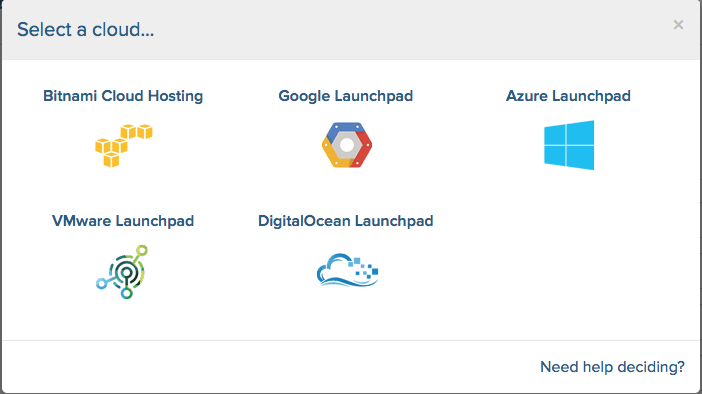
\includegraphics[width=\textwidth]{./03_Analyse/03_Bitnami/images/clouds}
\subsubsection{Bitnami Cloud Hosting}
Beim Bitnami Cloud Hosting steckt AWS dahinter, hier sind die meisten 
Einstellungen möglich im Vergleich zu den anderen Dashboards.


\textbf{Übersicht}
kurze Übersicht über die möglichen Konfigurationen einer AWS Instanz.
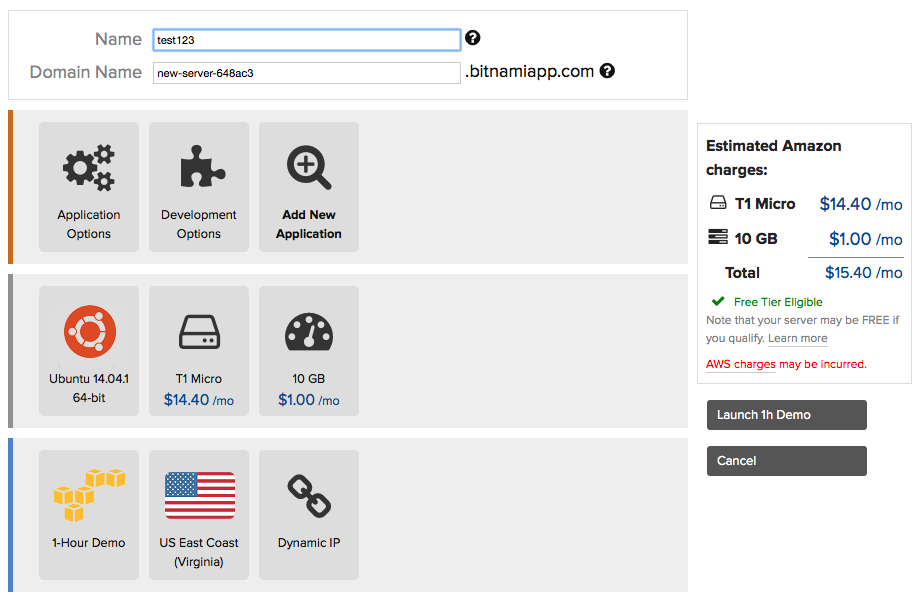
\includegraphics[width=0.8\textwidth]{./03_Analyse/03_Bitnami/images/aws_overview}
\newpage
\textbf{Application Options:}

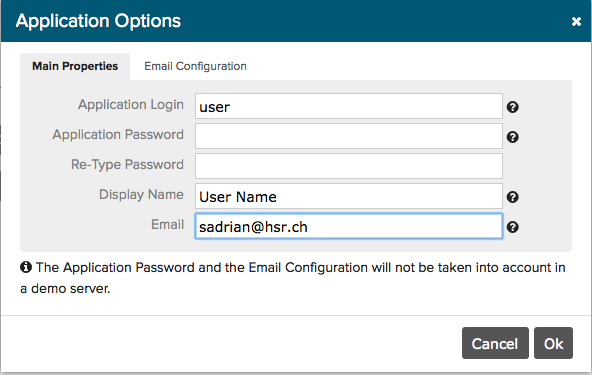
\includegraphics[width=0.5\textwidth]{./03_Analyse/03_Bitnami/images/aws_application_options}

\textbf{Applikationsauswahl:}

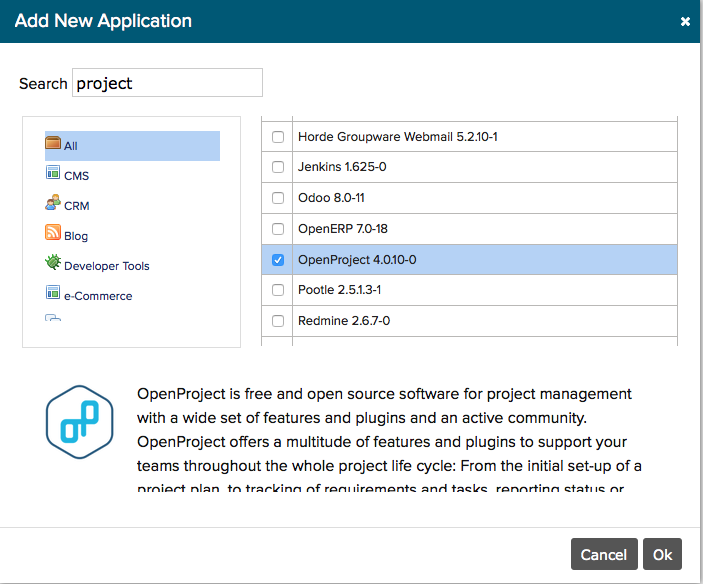
\includegraphics[width=0.5\textwidth]{./03_Analyse/03_Bitnami/images/aws_add_application}

\textbf{Betriebssystem:}

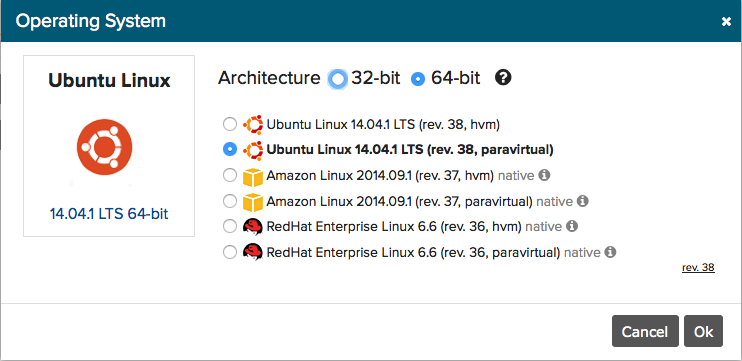
\includegraphics[width=0.5\textwidth]{./03_Analyse/03_Bitnami/images/aws_operating_system}

\textbf{Servertyp:}

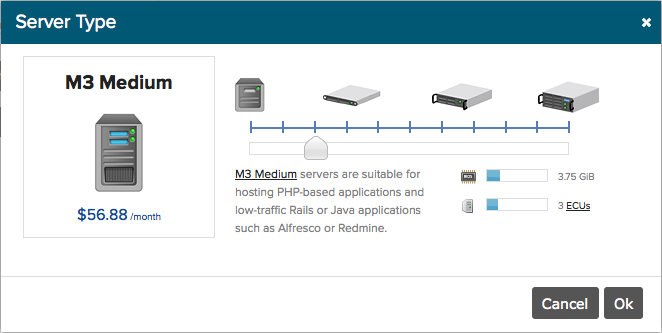
\includegraphics[width=0.5\textwidth]{./03_Analyse/03_Bitnami/images/aws_servertype}
\newpage
\textbf{Diskgrösse:}

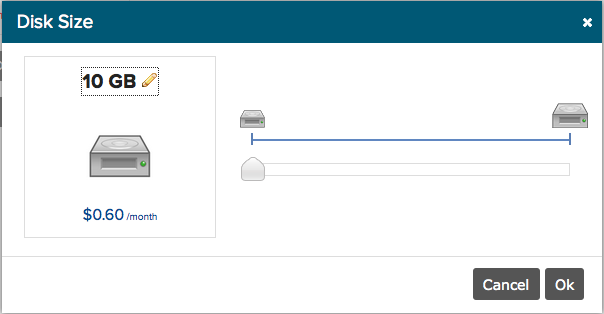
\includegraphics[width=0.5\textwidth]{./03_Analyse/03_Bitnami/images/aws_disk}

\textbf{Region,IP,Account:}

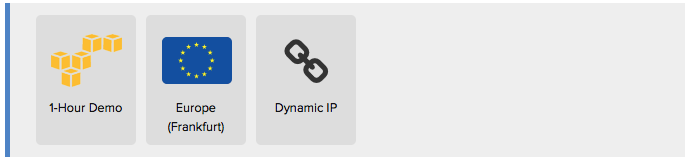
\includegraphics[width=0.5\textwidth]{./03_Analyse/03_Bitnami/images/aws_random}

\textbf{Management:}

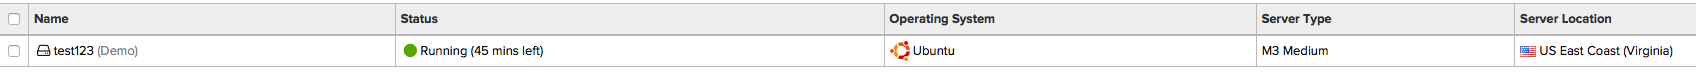
\includegraphics[width=\textwidth]{./03_Analyse/03_Bitnami/images/aws_overview_managment}

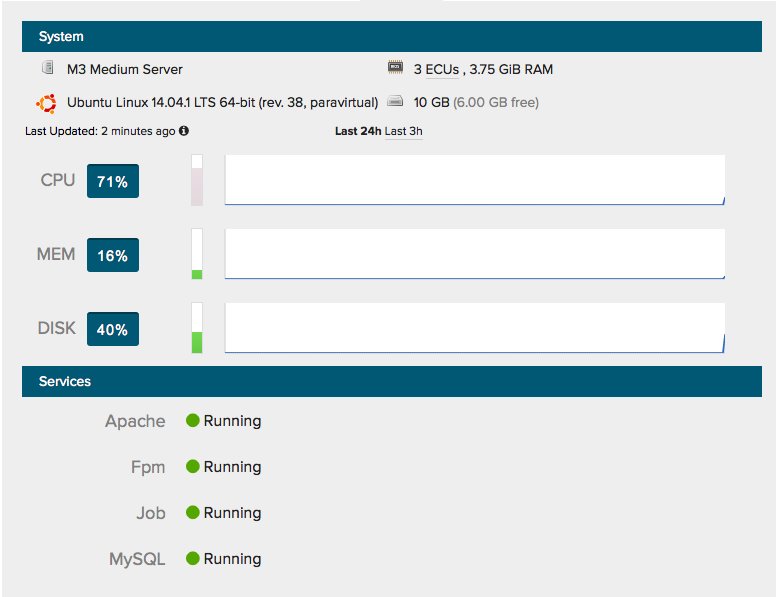
\includegraphics[width=0.5\textwidth]{./03_Analyse/03_Bitnami/images/aws_resourcen}

\textbf{Ressourcen:}

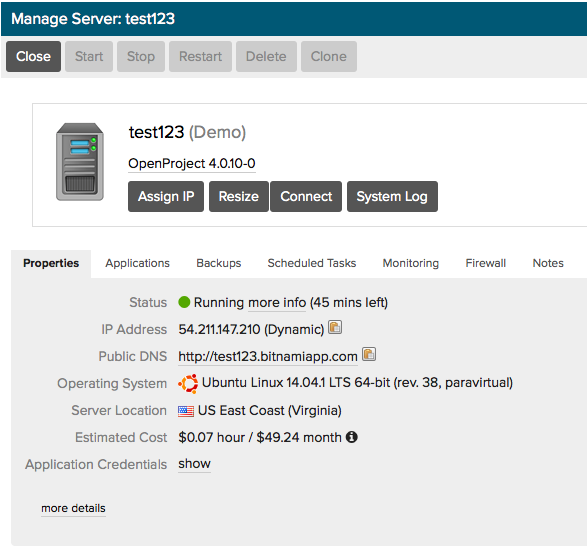
\includegraphics[width=0.5\textwidth]{./03_Analyse/03_Bitnami/images/aws_managment}

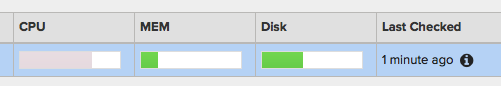
\includegraphics[width=0.5\textwidth]{./03_Analyse/03_Bitnami/images/aws_resrouces}

\newpage
\subsubsection{Digitalocean Launchpad}
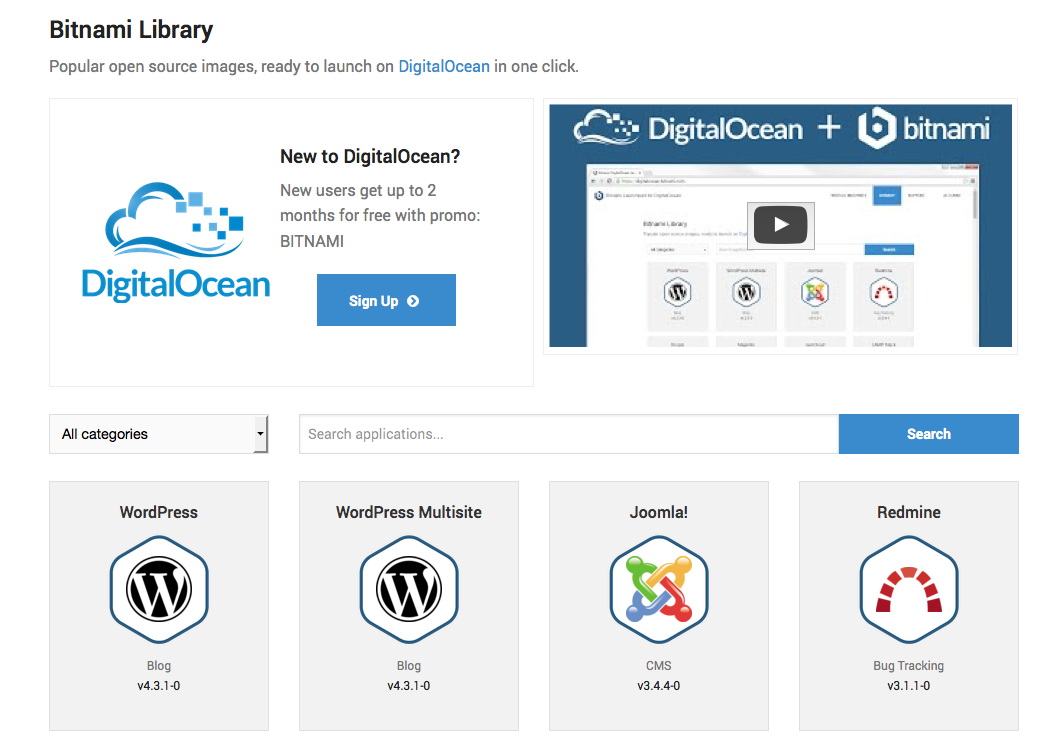
\includegraphics[width=\textwidth]{./03_Analyse/03_Bitnami/images/digitalocean_launchpad}
\textbf{Instanzen:}
Sobald eine Applikation ausgewählt wurde kann eine Instanz mit dem App gestartet 
werden, dabei kann noch die Instanzgrösse und Location gewählt werden.

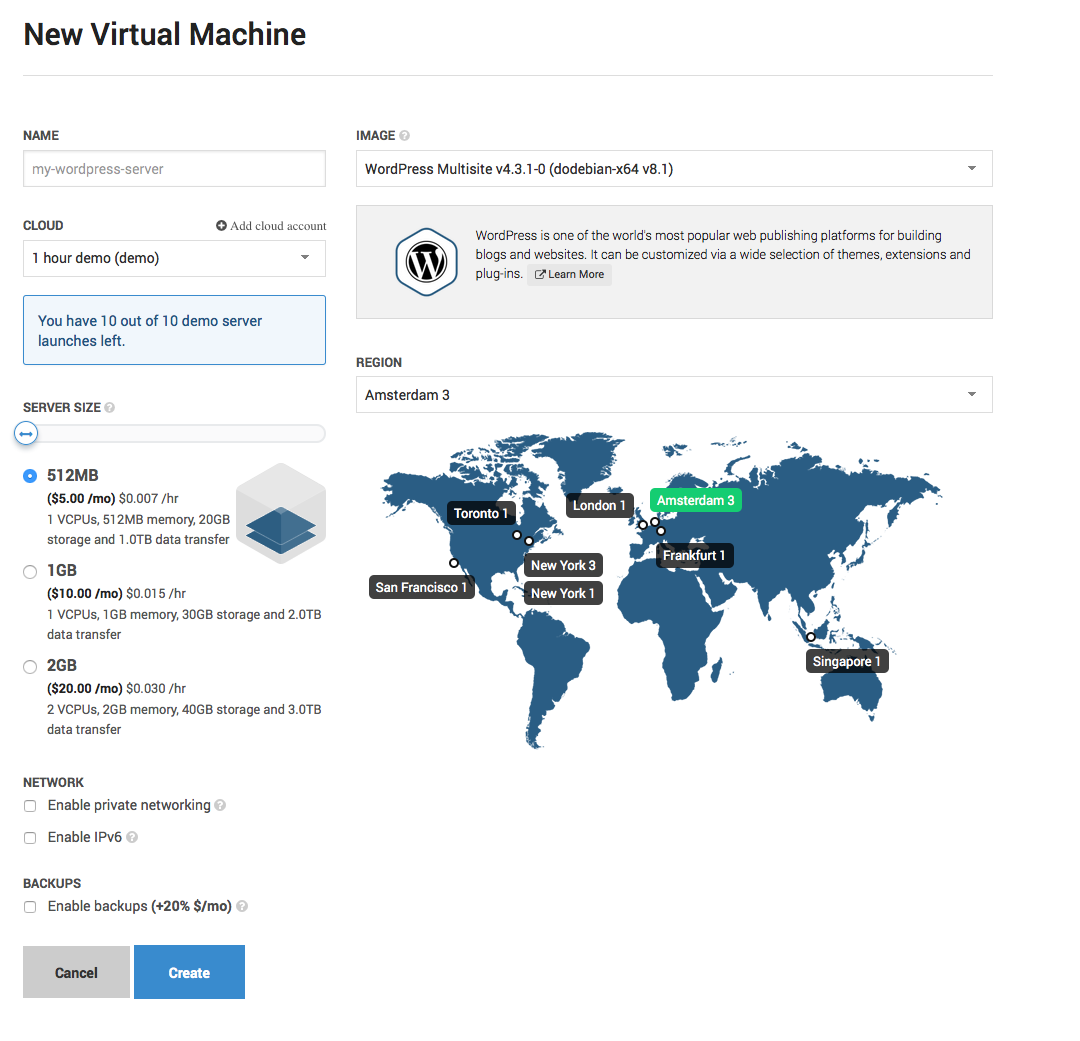
\includegraphics[width=\textwidth]{./03_Analyse/03_Bitnami/images/digitalocean_size}
Sobald Instanz erstellt lässt sich deren Status überprüfen + App spezifische 
Links werden gesetzt.

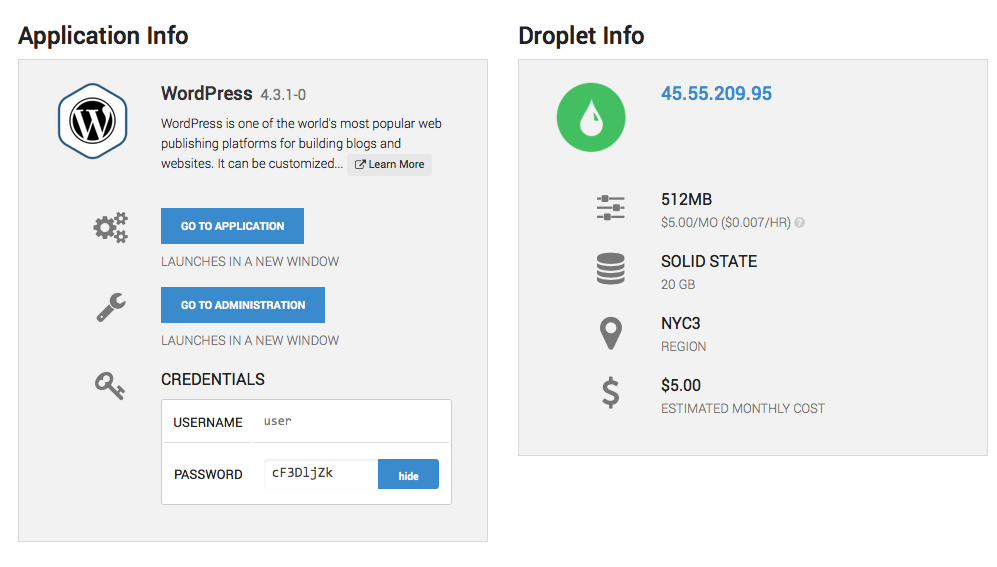
\includegraphics[width=\textwidth]{./03_Analyse/03_Bitnami/images/digitalocean_infos}

\textbf{Authorize Application:}
Um wirkliche Instanz erstellen zu können muss das Bitnami Dashboard Zugriff auf 
den Cloud spezifischen Account haben.

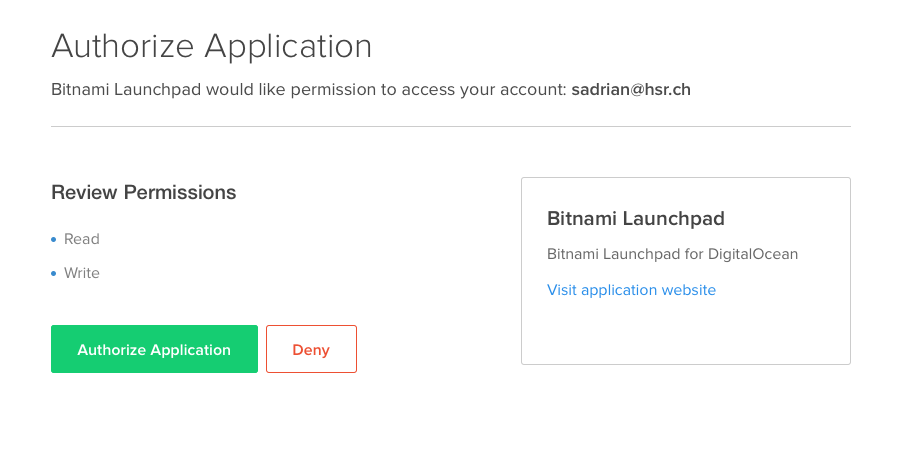
\includegraphics[width=\textwidth]{./03_Analyse/03_Bitnami/images/digitalocean_authorize}

Dabei können mehrere Accounts hinzugefügt werden:

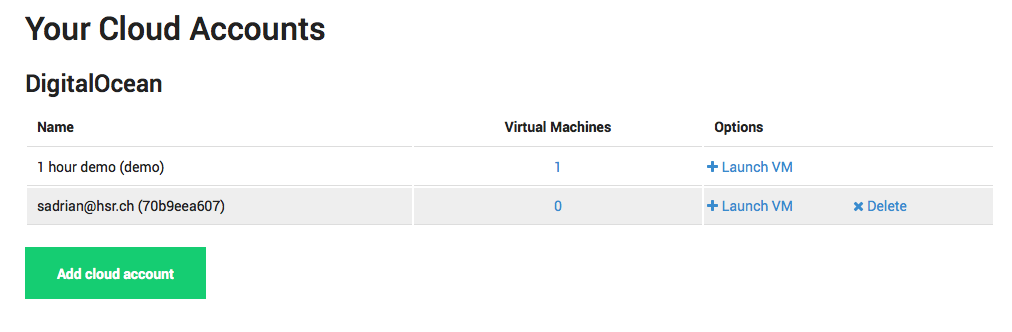
\includegraphics[width=\textwidth]{./03_Analyse/03_Bitnami/images/digitalocean_accounts}

Und unter jedem Account können spezifisch VM's erstellt werden:

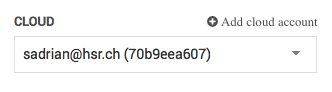
\includegraphics[width=0.4\textwidth]{./03_Analyse/03_Bitnami/images/digitalocean_account_specific}

Danach taucht die Instanz in der Übersicht auf:

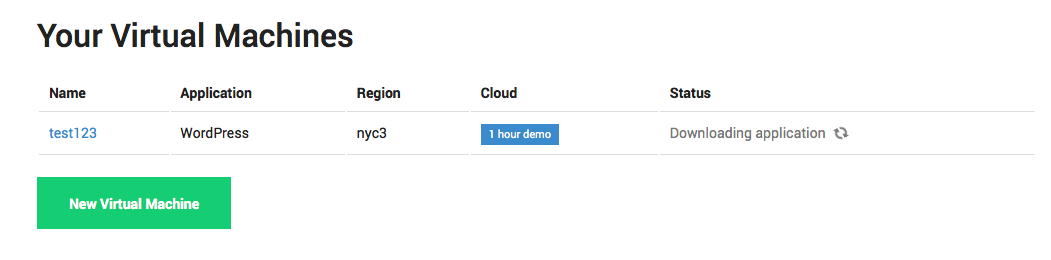
\includegraphics[width=\textwidth]{./03_Analyse/03_Bitnami/images/digitalocean_instances}

\newpage
\textbf{Instanzinfos:}

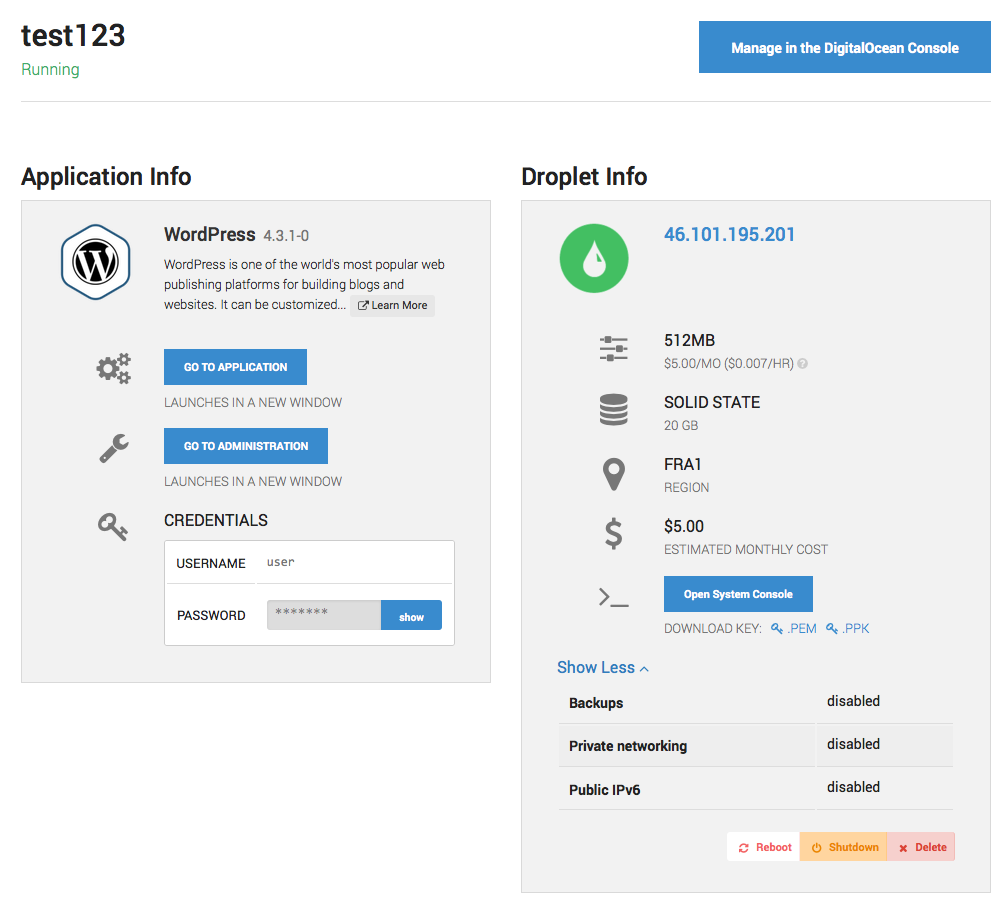
\includegraphics[width=\textwidth]{./03_Analyse/03_Bitnami/images/digitalocean_instanceinfo}

\subsubsection{Azure Launchpad}
Beim Azure Launchpad wird wieder gleich vorgegangen, wie bei Digitalocean.
Nur das sich die infos ändern (Bspw.: Bei Digitalocean Droplet, jetzt Server).

Ebenfalls ändern sich die Instanzgrössen. welche bei Azure anders als bei 
Digitalocean sind + wird bei Azure mit Subscriptions und nicht anhand von 
Accounts unterschieden.
\textbf{Serverinfo:}

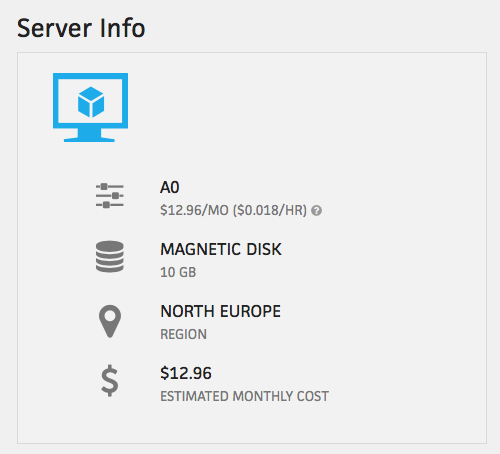
\includegraphics[width=0.5\textwidth]{./03_Analyse/03_Bitnami/images/azure_serverinfo}

\textbf{Authorization:}

Bei Azure wird das Dashboard über ein Managment Certificate autorisiert:

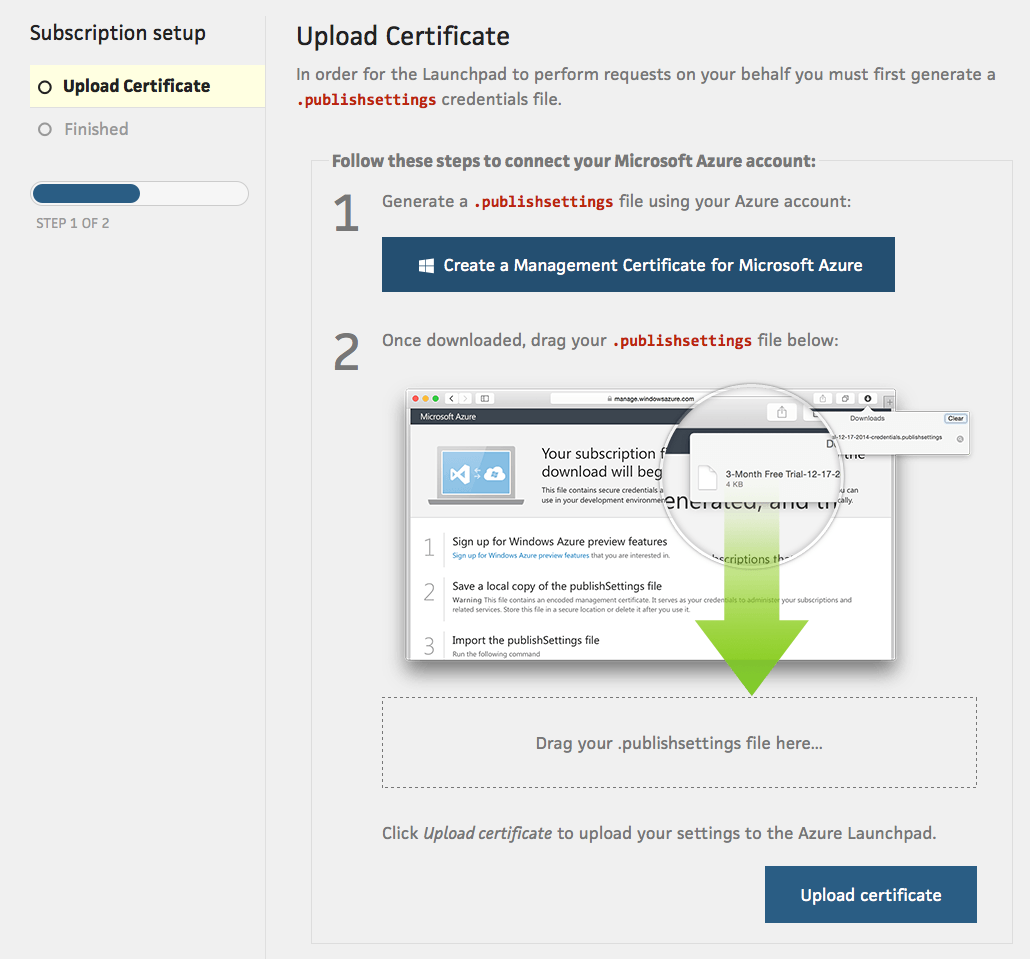
\includegraphics[width=0.8\textwidth]{./03_Analyse/03_Bitnami/images/azure_authorize}

Danach wird die vorhandene Subscription/s vom Microsoft Account eingebunden:

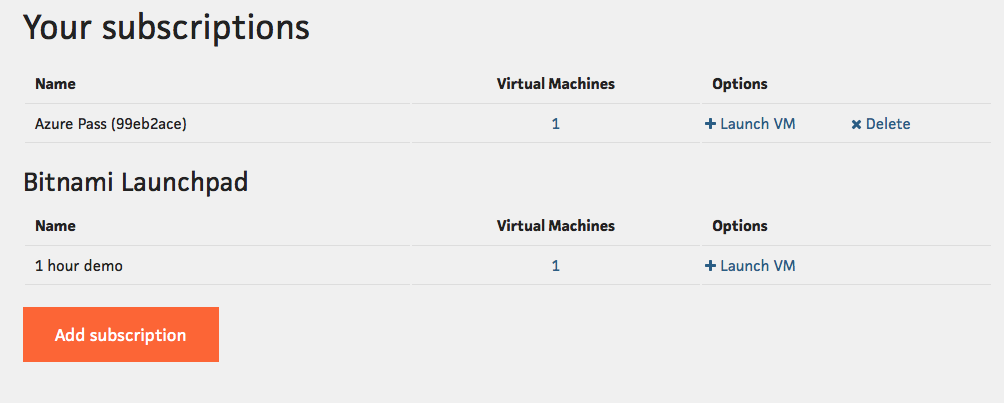
\includegraphics[width=0.8\textwidth]{./03_Analyse/03_Bitnami/images/azure_subscriptions}


Sobald dann ein neuer Server erstellt wurde kann dieser auch wieder gelöscht 
werden und all dessen Infos angesehen werden.

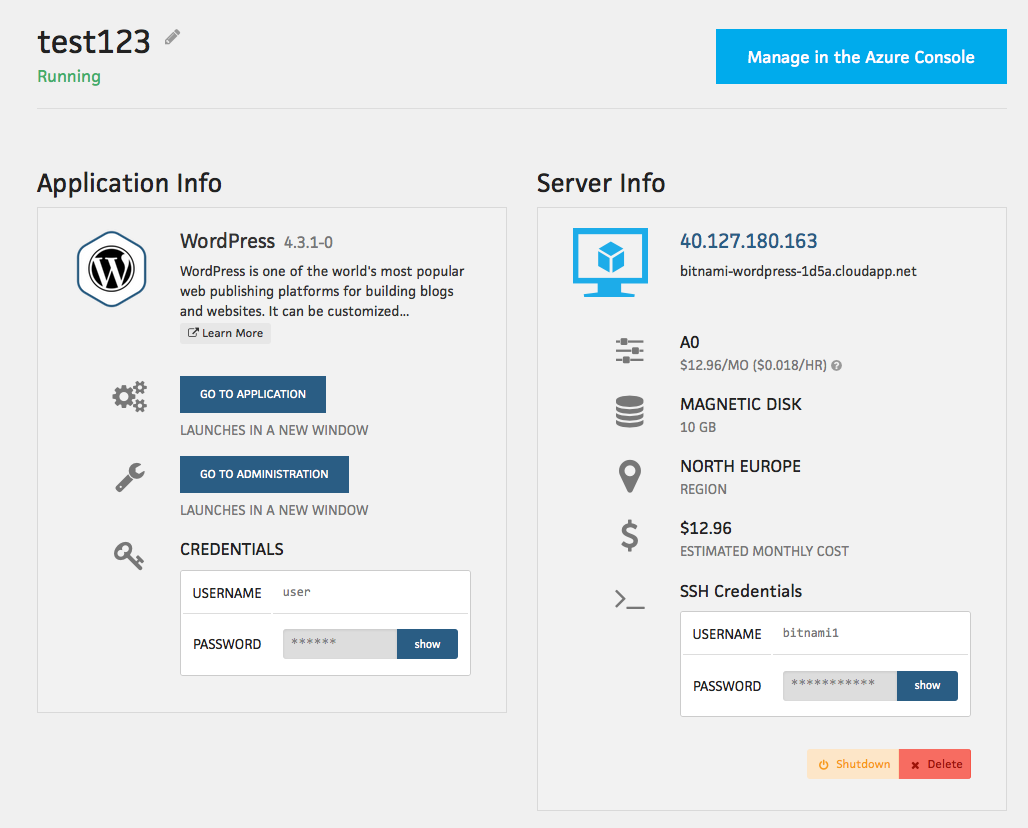
\includegraphics[width=0.8\textwidth]{./03_Analyse/03_Bitnami/images/azure_instanceinfos}

\subsubsection{Google Launchpad}

Beim Google Launchpad wieder dasselbe, wie bei Azure oder Digitalocean.
Hier wird einfach mit Projekten unterschieden (schliesslich kann jedem Projekt mehrere Compute Instanzen 
oder andere Services angefügt sein.)


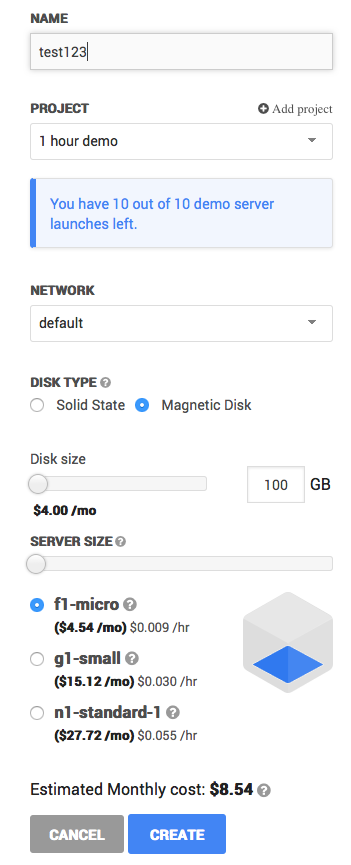
\includegraphics[width=0.4\textwidth]{./03_Analyse/03_Bitnami/images/google_instancereation}


\subsubsection{VMware Launchpad}
Das VMware Launchpad kann für die WMware vCloud Air gebraucht werden.

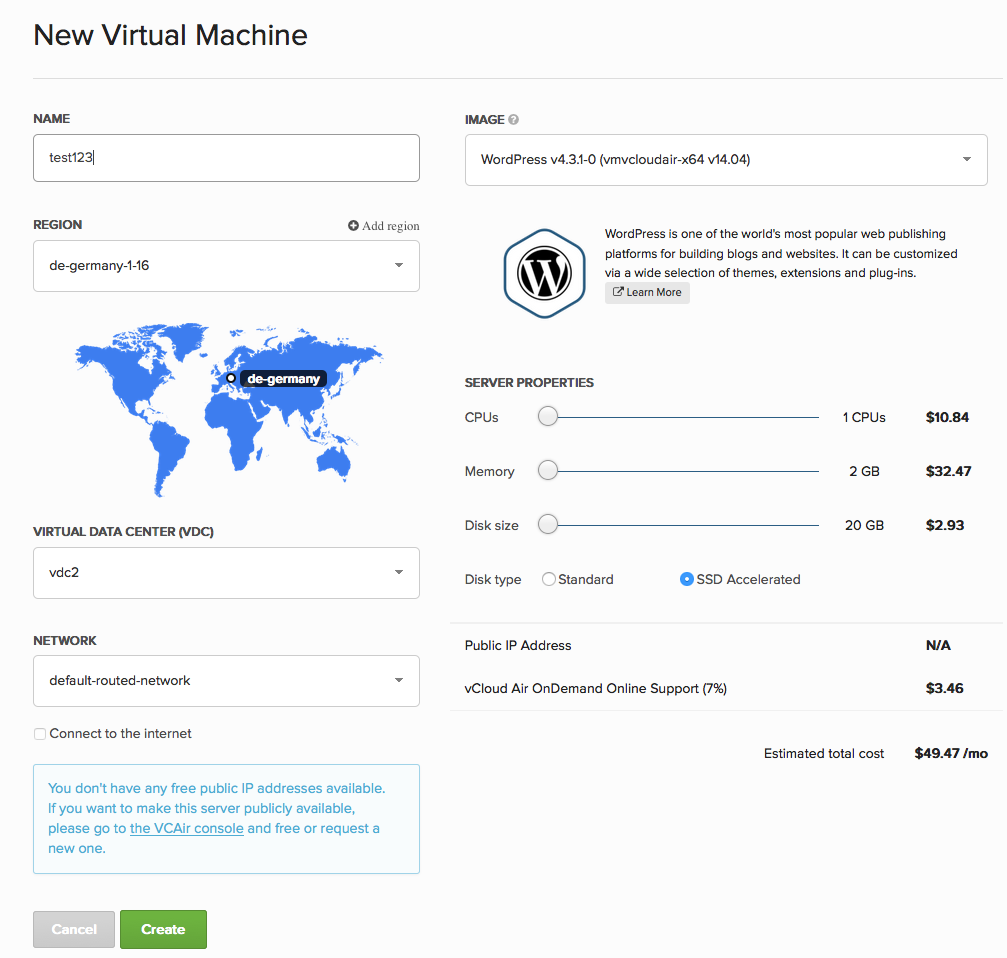
\includegraphics[width=0.8\textwidth]{./03_Analyse/03_Bitnami/images/vmware_creation}

\textbf{Infos:}

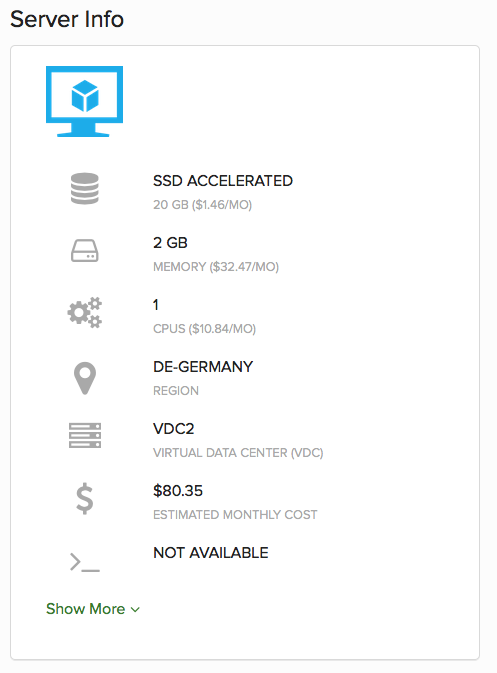
\includegraphics[width=0.4\textwidth]{./03_Analyse/03_Bitnami/images/vmware_infos}

\subsection{Security}
Da durch das zentrale zusammenfassen von mehreren Accounts auch immer 
Sicherheitsrisiken zu beachten sind, wird bei Bitnami zusätzlich zum normalen 
Loginpasswort auch noch ein Vaultpasswort festgelegt, welches wohl die 
Logindaten symmetrisch verschlüsselt und in einem ``Vault'' ablegt.

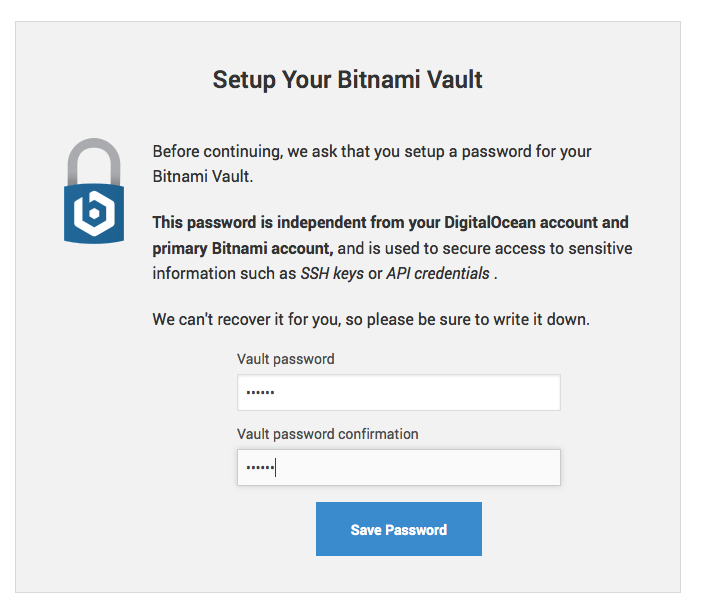
\includegraphics[width=0.8\textwidth]{./03_Analyse/03_Bitnami/images/bitnami_security}

\subsection{Applikationen}
Die Applikationen können sich von Anbieter zu Anbieter unterscheiden, jedoch 
gibt es für sehr viel verwendete Applikationen (Bspw.: Wordpress) bei jedem ein 
Image.
Es besteht bereits eine sehr grosse Auswahl für sehr viel verschiedene Apps und 
es werden immer mehr, wodurch es immer einfacher wird schnell eine Applikation 
aufzusetzen.
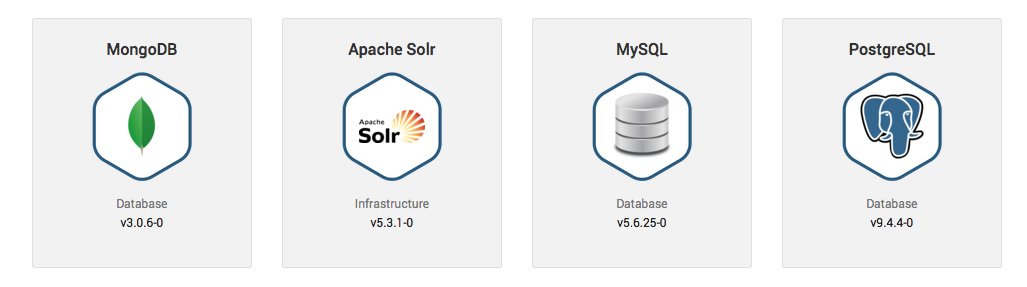
\includegraphics[width=\textwidth]{./03_Analyse/03_Bitnami/images/apps}

\subsubsection{Kategorien}
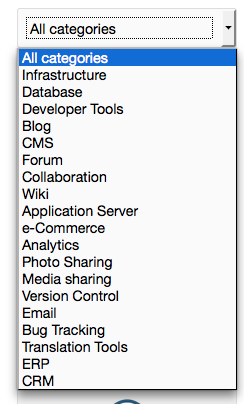
\includegraphics[width=0.3\textwidth]{./03_Analyse/03_Bitnami/images/categories}

\section{Fazit}
Bitnami bietet einiges was Computing angeht und ist der einzig grössere 
Dashboard Anbieter, der mehrere verschiedene Cloud Anbieter unterstützt.
Allerdings fehlen verschiedene PaaS Angebote (Bspw.: Cloud SQL bei Google etc.), 
Bitnami ist daher nur für eigene Instanzen/Vms zu gebrauchen und nicht mit einer 
generellen Service Unterstützung konzipiert worden.
Das Dashboard bei Bitnami bietet jedenfalls einiges und gibt einem einen guten 
Überblick über seine eigenen abonnierten Services (VM Instanzen).

\newpage
\section{Dashboard}
Das Dashboard soll dem Nutzer schnell und einfach die Übersicht über seine 
eigenen abonnierten Services bieten (Compute,Storage,Network).
Dabei soll auf eine Anzahl von Cloud Anbietern angeboten werden, sowohl Public 
Cloud(z.B.: AWS, Google Cloud, Azure, Digitalocean), wie auch Private Cloud (z.B.:CloudStack.Open 
Stack).
Die nachfolgenden Mockups sollen bereits einen ersten Eindruck der 
möglichen Funktionalitäten des Dashboard geben.
\\
\textbf{Beim Login wird zwischen Nutzern und Administrator unterschieden.}

\subsection{Homescreen Nutzer}
Der Nutzer kriegt eine Übersicht über die vorhanden Cloud Anbieter und kann 
gemäss Wunsch den richtigen wählen.
\begin{figure}[!htbp]
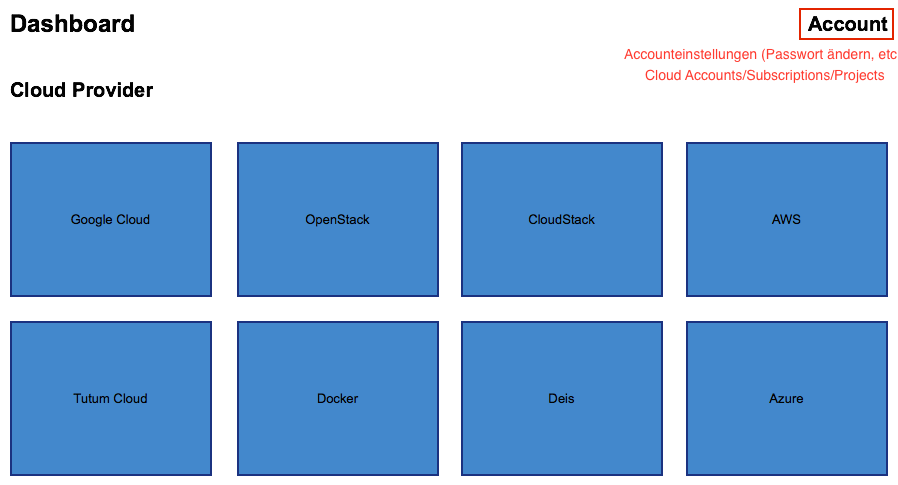
\includegraphics[width=\textwidth]{./03_Analyse/03_Dashboard/images/homescreen_user}
\caption{Homescreen Nutzer}
\end{figure}

\newpage

\subsection{Homescreen Admin}

Der Administrator kriegt lediglich eine Übersicht über die vorhanden Nutzer und 
kann diese löschen oder ändern.
\begin{figure}[!htbp]
  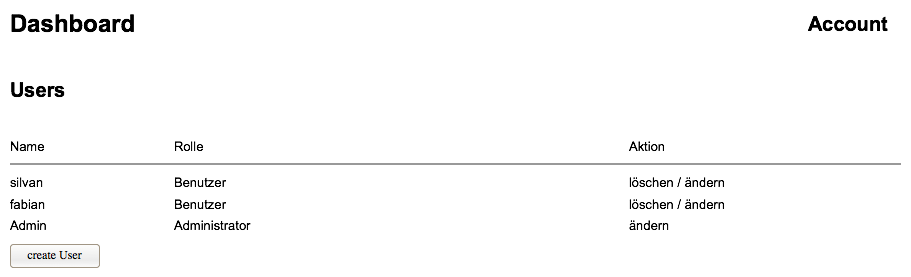
\includegraphics[width=\textwidth]{./03_Analyse/03_Dashboard/images/homescreen_admin}
  \caption{Homescreen Admin}
\end{figure}


\subsection{Offerings}
Sobald man einer der Cloud Anbieter gewählt hat (auf dem Homescreen) öffnet 
sich das jeweilige Dashboard des Anbieters mit dessen spezifischen Services.
\begin{figure}[!htbp]
  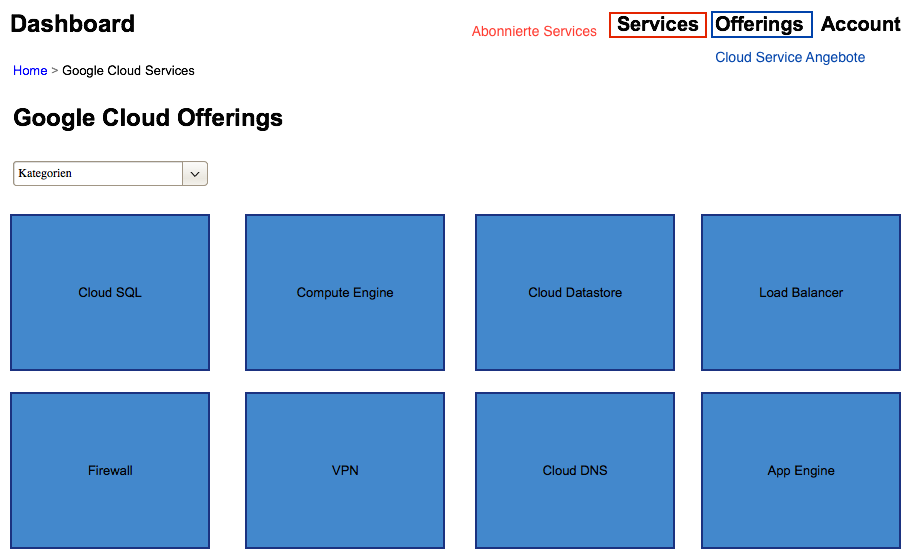
\includegraphics[width=\textwidth]{./03_Analyse/03_Dashboard/images/homescreen_google}
  \caption{Homescreen Google}
\end{figure}

\newpage

   \subsubsection{Compute:}
Hier werden nur Compute Offerings angezeigt z.B.: App Engine, Compute Engine, 
Container Engine, EC2 etc., können nach Anbieter variieren

\begin{figure}[!htbp]

   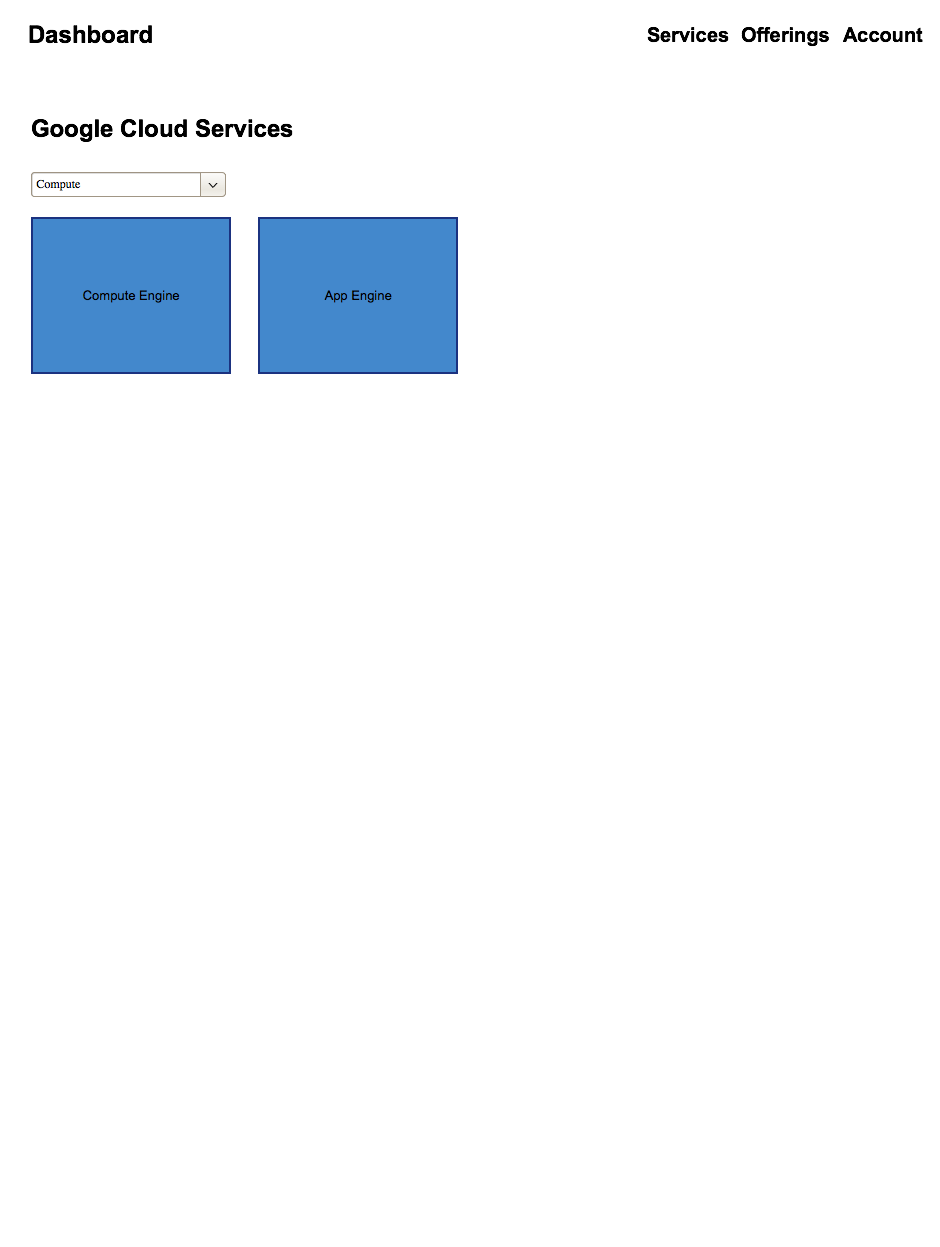
\includegraphics[width=\textwidth]{./03_Analyse/03_Dashboard/images/homescreen_google_compute}
   \caption{Homescreen Kategorie Compute}
\end{figure}
 

\subsubsection{Storage:}

Nur Storage spezifische Offerings anzeigen z.B.: Cloud Datastore, Cloud SQL, 
Cloud BigTable), die sich je nach Anbieter ändern. 
\begin{figure}[!htbp]
 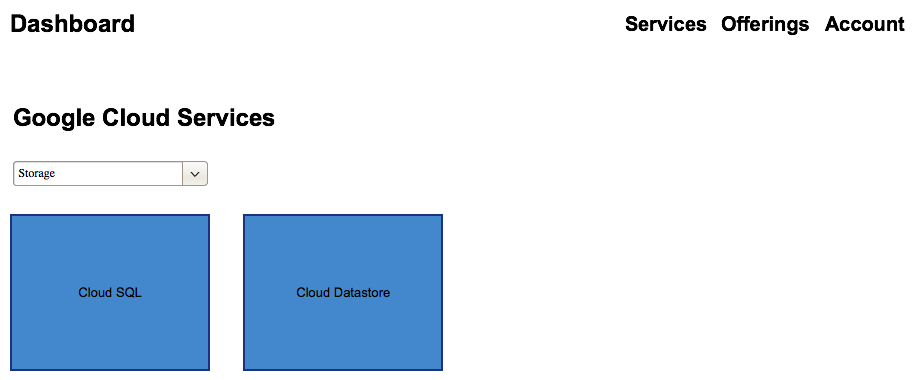
\includegraphics[width=\textwidth]{./03_Analyse/03_Dashboard/images/homescreen_google_storage}
  \caption{Homescreen Kategorie Storage}
\end{figure}

\subsubsection{Network:}
Network spezifische Offerings anbieten (Firewall, VPN, Netzwerke, Cloud DNS etc.) 
und dann verändert sich die Auswahl auch Anbieter spezifisch. 

\begin{figure}[!htbp]
 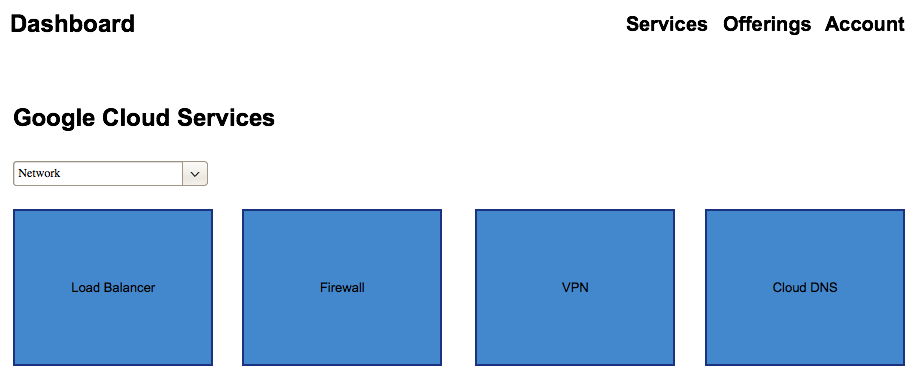
\includegraphics[width=\textwidth]{./03_Analyse/03_Dashboard/images/homescreen_google_network}
    \caption{Homescreen Kategorie Network}
\end{figure}

\newpage

\subsection{Services}
In Services kriegt man einen Überblick über all seine abonnierten Services des jeweiligen 
Anbieters und kann den zu bearbeitenden wählen.
\begin{figure}[!htbp]
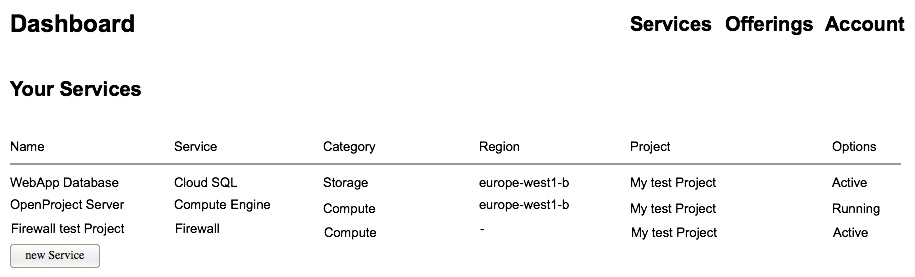
\includegraphics[width=\textwidth]{./03_Analyse/03_Dashboard/images/services_overview}
\caption{Services Übersicht}
\end{figure}

\subsubsection{Compute}
Wenn man einen Compute Service wählt kriegt man eine Übersicht des Services, 
welcher Storage, Leistung + Region (Storage und Compute werden jedoch 
meistens vorgegeben durch die Instanzgrössen) + werden die Kosten pro 
Monat angezeigt.
Im Management kann dann die Instant direkt neugestartet/heruntergefahren oder gelöscht 
werden + sollen noch Links (Ip etc.) zur Verfügung stehen um sich auf die Instanz 
 verbinden zu können.
 
\begin{figure}[!htbp]
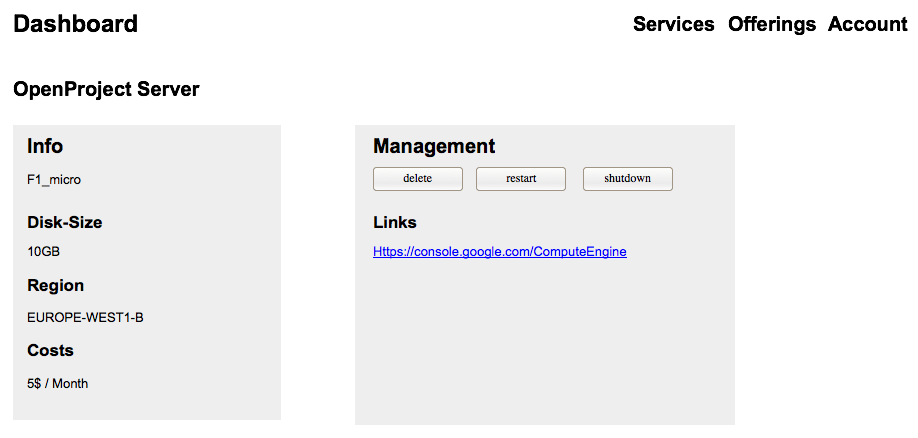
\includegraphics[width=\textwidth]{./03_Analyse/03_Dashboard/images/service_info_compute}
\caption{Services Infos Compute}
\end{figure}

\subsubsection{Storage}
Bei Storage spielt es wieder eine Rolle was für eine Art Storage es ist in 
diesem Beispiel ist es eine Cloud SQL Datenbank.
Dabei wird vielmals anhand der Anzahl Rows oder Grösse der Datenbank abgerechnet 
+ sollen hier auch wieder Links verfügbar sein, um auf ein Datenbankdashboard zu 
gelangen + die Möglichkeit geben den Service löschen zu können.

\begin{figure}[!htbp]
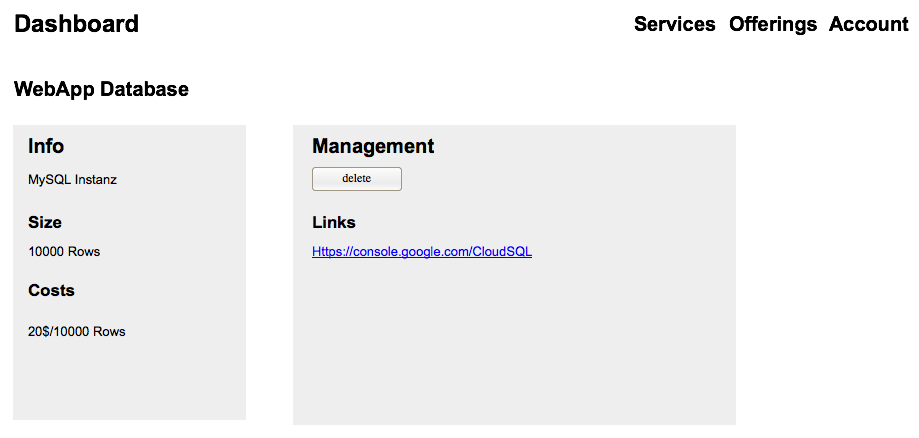
\includegraphics[width=0.8\textwidth]{./03_Analyse/03_Dashboard/images/service_info_storage}
\caption{Services Infos Storage}
\end{figure}

\subsubsection{Network}
Bei Network kann man noch einige Dinge konfigurieren von Cloud DNS bis zu 
Netzwerken (Subnetze etc.) auch Firewall Regeln, da bei den Cloud Anbietern 
vielmals nur SSH und HTTP/S zugelassener traffic ist muss man schliesslich auch 
die Möglichkeit haben Firewall Regeln festlegen zu können.
Das könnte Schlussendlich in etwa so aussehen:

\begin{figure}[!htbp]
  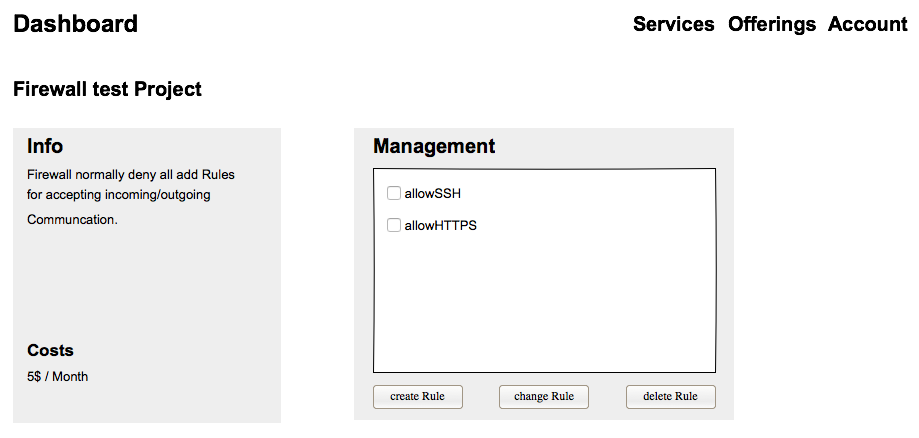
\includegraphics[width=0.8\textwidth]{./03_Analyse/03_Dashboard/images/service_info_network}
  \caption{Services Infos Network}
\end{figure}

\newpage

\subsection{Accounts/Subscriptions/Projects/...}
Für jeden Anbieter soll dem User eine Übersicht über die 
Account/Subscriptions/Projects gegeben werden, dadurch vereinfacht sich die 
Handhabung von mehreren Accounts und alle sind in einem Dashboard zusammengefügt 
(-> Security beachten).
Dadurch hat man immer den Überblick für welches Projekt/Account man wie viele 
Services abonniert hat.

\begin{figure}[!htbp]
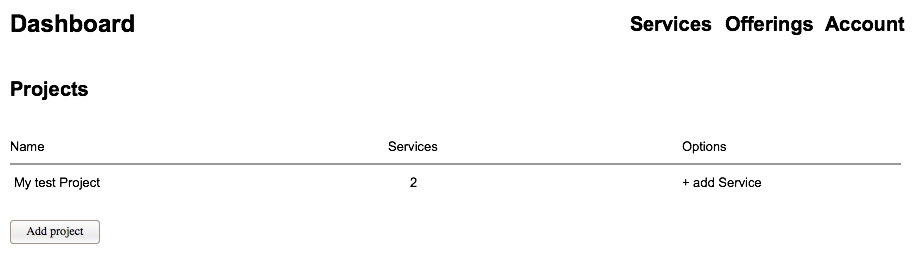
\includegraphics[width=\textwidth]{./03_Analyse/03_Dashboard/images/account_projects.png}
\caption{Accounts Übersicht}
\end{figure}

\section{Security}
Wie bei Bitnami wäre es wohl sicherer die Zugriffsdaten für die Cloud Anbieter 
abzusichern (bei Bitnami wird dies über ein Vault sichergestellt), ansonsten 
könnte ein Angreifer ganze Instanzen bei verschiedenen Anbietern löschen oder 
sonstige Bösartige Absichten ausüben.

Dieser Vault soll auch durch ein zusätzliches Passwort geschützt sein und 
wird symmetrisch verschlüsselt (Mail Anbieter: Proton Mail\autocite{proton} macht dies ebenfalls 
so) -> jedoch fragt Bitnami bei jedem login wieder nach dem Passwort und 
vergisst dann wieder alle Instanzen (ein Abgleich mit dem Anbieter wäre hier sicher nicht 
schlecht).

\newpage

\section{Fazit}
Das Servicedashboard scheint soweit umsetzbar zu sein, ein Knackpunkt wird 
einfach noch die Absicherung der Zugriffe auf alle die Cloud Anbieter und deren 
Services.
Z.B.: Bitnami bietet ein Download für Private Key und Putty Key File an:
\begin{figure}[!htbp]
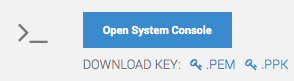
\includegraphics[width=0.5\textwidth]{./03_Analyse/03_Dashboard/images/bitnami_private_key}
\caption{Bitnami Private Key}
\end{figure}
Und erstellt für jeden Server ein neues keypaar:
\begin{figure}[!htbp]
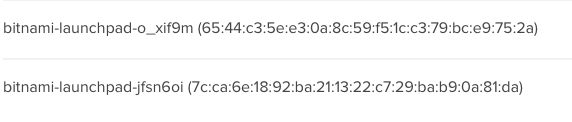
\includegraphics[width=0.5\textwidth]{./03_Analyse/03_Dashboard/images/bitnami_key}
\caption{Bitnami Key}
\end{figure}
Was nicht gerade die Beste Lösung ist.


\documentclass[11pt]{scrartcl}

\title{Use Case Skizzen}
\author{Silvan Adrian \\ Fabian Binna}
\date{\today{}}

\usepackage[ngerman]{babel}
\usepackage[automark]{scrpage2}
\usepackage{hyperref}
\usepackage{color}
\usepackage[normalem]{ulem}
\usepackage{scrpage2}
\usepackage{graphicx}
\usepackage{tabularx}
\graphicspath{ {../22_Grafiken/01_Logo/}{images/}{../../22_Grafiken/01_Logo/} }
\pagestyle{scrheadings}

\clearscrheadfoot
\ihead{
\includegraphics[scale=0.3]{SDDC}}
\ohead{Projekt: SDDC}
\ifoot{Use Case Skizzen}
\cfoot{Version: 1.01}
\ofoot{Datum: \today{}}
\setheadsepline{0.5pt}
\setfootsepline{0.5pt}

\usepackage{ucs}
\usepackage[utf8]{inputenc}
\usepackage[T1]{fontenc}


\begin{document}
\def\arraystretch{1.5}
\begin{titlepage}
\begin{center}
\vspace{10em}

\includegraphics[scale=2]{SDDC}
\vspace{10em}
\end{center}
\begin{center}
\huge {Template}
\end{center}
\begin{center}
\vspace{10em}
\LARGE {Silvan Adrian} \\
\LARGE {Fabian Binna}
\end{center}

\end{titlepage}

\newpage
\section{Änderungshistorie}
\begin{tabularx}{\linewidth}{l l X l}
\textbf{Datum} & \textbf{Version} & \textbf{Änderung}  & \textbf{Autor} \\
\hline
\textbf{25.09.15} & 1.00 & Erstellung des Dokuments & Gruppe \\
\textbf{25.06.15} & 1.01 & Aktoren und Use Cases aus dem Diagramm & Silvan 
Adrian\\
\textbf{27.09.15} & 1.02 & Diagramm eingefügt + Verbesserungen & Silvan Adrian\\
\end{tabularx}

\newpage
\tableofcontents
\newpage
\section{Akteure}
\begin{tabularx}{\linewidth}{X X}
\textbf{Akteur} & \textbf{Ziel}\\
\hline
\textbf{Public User} &
Registrieren
\\
\hline
\textbf{Registered User} & 
\textbf{Wenn User:}

Login

Logout

Service anlegen (Create)

Service Infos lesen (Read)

Service ändern (Update)

Service löschen (Delete)

Benutzerinfos ändern

\textbf{Wenn Admin:}

Benutzer anlegen

Benutzer löschen

Benutzer ändern

Benutzerinfos ändern

\\
\hline
\textbf{Cloud Anbieter} &
Service anlegen (Create)

Service Infos lesen (Read)

Service ändern (Update)

Service löschen (Delete)
\\

\end{tabularx}


\section{Use Case Diagramm}

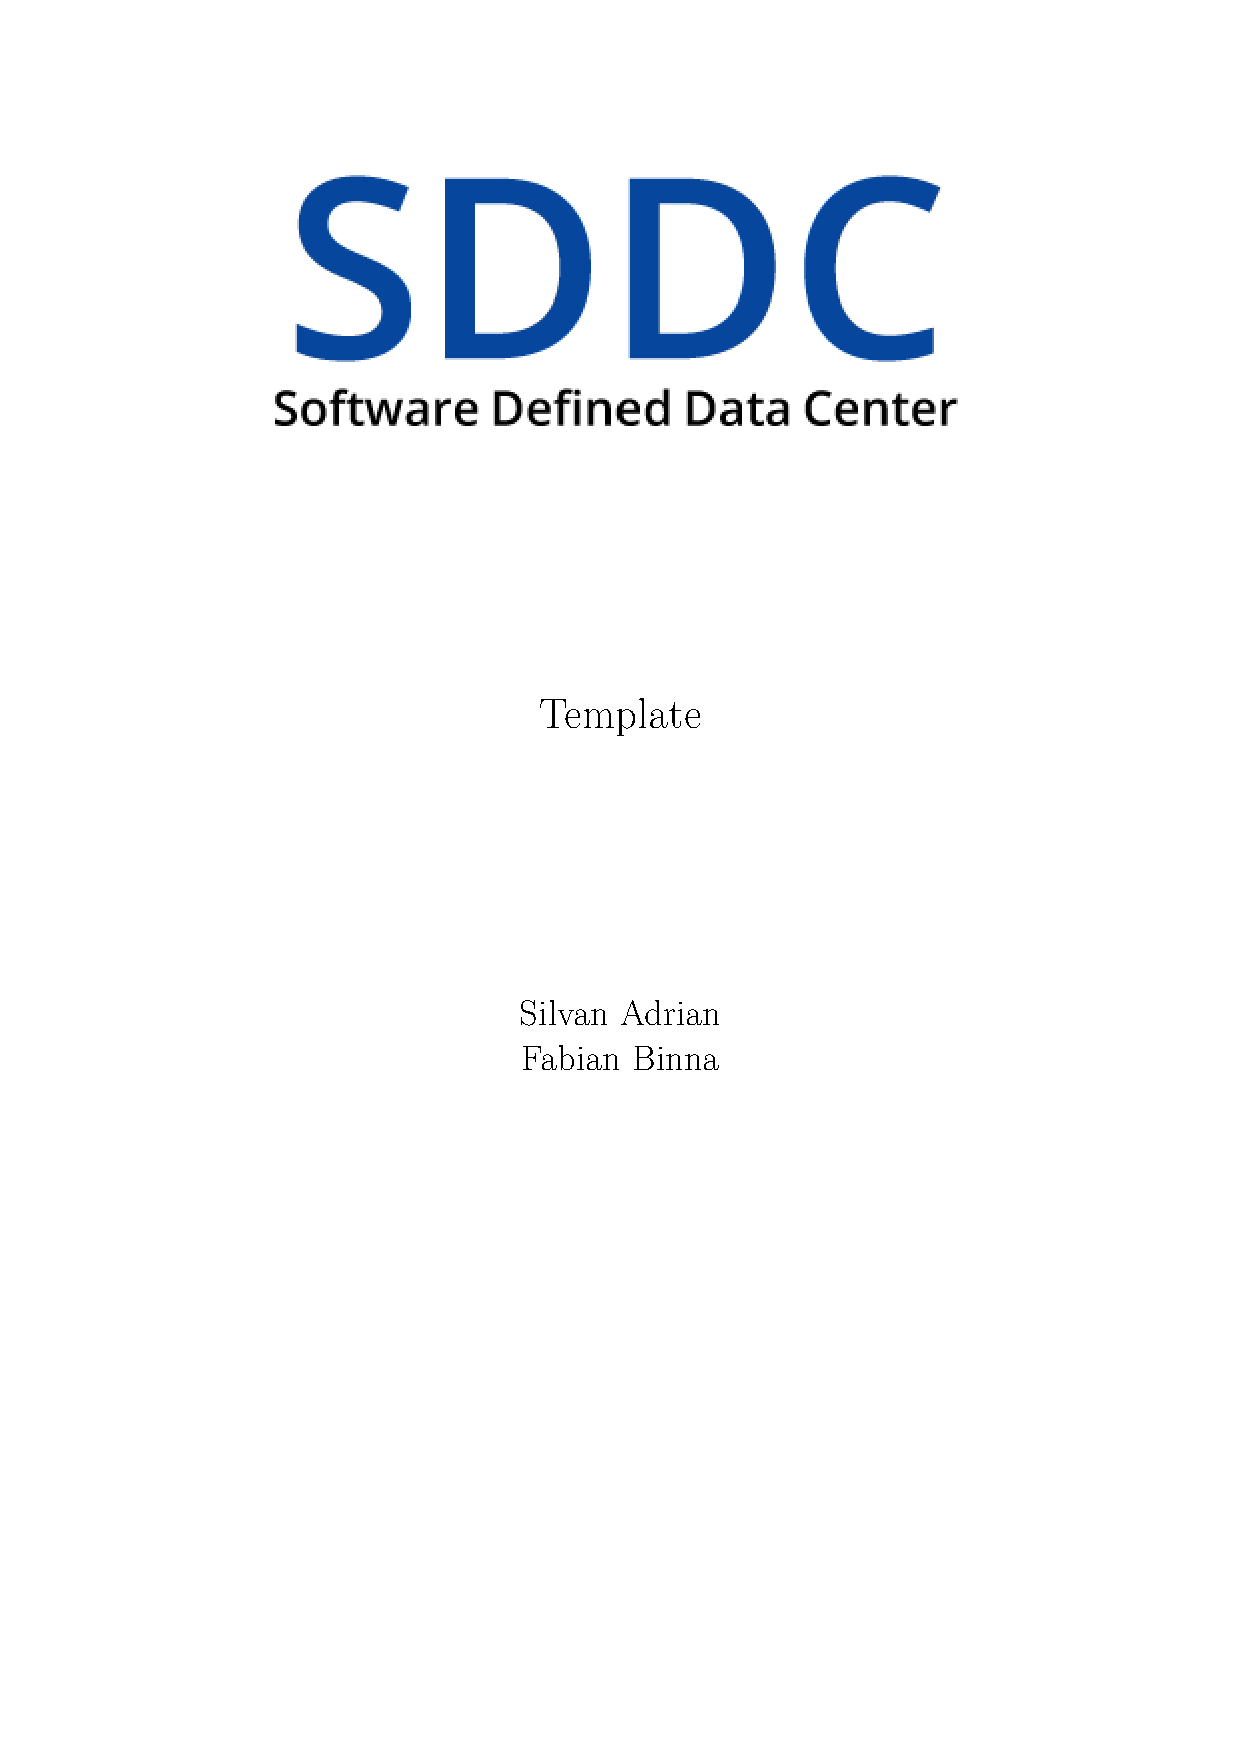
\includegraphics[width=\textwidth]{UseCase-Skizzen}



\end{document}
\documentclass[11pt]{scrartcl}

\title{User Stories Skizzen}
\author{Silvan Adrian \\ Fabian Binna}
\date{\today{}}

\usepackage[ngerman]{babel}
\usepackage[automark]{scrpage2}
\usepackage[colorlinks = true,
linkcolor = black]{hyperref}
\usepackage{color}
\usepackage[normalem]{ulem}
\usepackage{scrpage2}
\usepackage{graphicx}
\usepackage{tabularx}
\graphicspath{ {../22_Grafiken/01_Logo/}{images/}{../../22_Grafiken/01_Logo/} }
\pagestyle{scrheadings}

\clearscrheadfoot
\ihead{
\includegraphics[scale=0.3]{SDDC}}
\ohead{Projekt: SDDC}
\ifoot{User Stories Skizzen}
\cfoot{Version: 1.02}
\ofoot{Datum: \today{}}
\setheadsepline{0.5pt}
\setfootsepline{0.5pt}

\usepackage{ucs}
\usepackage[utf8]{inputenc}
\usepackage[T1]{fontenc}


\begin{document}
\def\arraystretch{1.5}
\begin{titlepage}
\begin{center}
\vspace{10em}
\includegraphics[scale=2]{SDDC}
\vspace{10em}
\end{center}
\begin{center}
\huge {User Stories Skizzen}
\end{center}
\begin{center}
\vspace{10em}
\LARGE {Silvan Adrian} \\
\LARGE {Fabian Binna}
\end{center}

\end{titlepage}

\newpage
\section{Änderungshistorie}
\begin{tabularx}{\linewidth}{l l X l}
\textbf{Datum} & \textbf{Version} & \textbf{Änderung}  & \textbf{Autor} \\
\hline
\textbf{26.09.15} & 1.00 & Erstellung des Dokuments & Gruppe \\
\textbf{26.09.15} & 1.01 & Einführung + Rollen & Silvan Adrian \\
\textbf{27.09.15} & 1.02 & Ziele + kurze User Stories Skizzen & Silvan Adrian\\
\end{tabularx}

\newpage
\tableofcontents
\newpage
\section{Einführung}

\subsection{Zweck}

Dieses Dokument beinhaltet die ersten Skizzen der User Stories.

\subsection{Gültigkeitsbereich}

Dieses Dokument ist während des ganzen Projekts gültig.


\subsection{Referenzen}
Bitnami-Analyse.pdf\\
Dashboard-Analyse.pdf\\
UseCase-Skizzen.pdf

\section{Rollen}
\subsection{Public User}
Public User sind alle öffentlichen Besucher des Dashboards.

\subsection{Registered User}
Der registrierte Nutzer ist Anwender des Dashboards und verwendet dieses zur 
Aufgabenerleichterung.
Bei dem Nutzer kann es sich um einen System Administrator, DevOps, Operator oder
Software Entwickler handlen, da beim Dashboard für jeden was dabei ist.

\subsection{Admin}
Der Admin ist für die Instandhaltung des Dashboards zuständig und verwaltet die 
User.

\section{Ziele}
Im Umfang soll die Applikation in etwa folgendes bieten:
\begin{itemize}
  \item Registrierung (Mail Adresse/Passwort)
  \item Login
  \item Administrationoberfläche
  \item Benutzerinfos anpassen
  \item Auswahl aus mehreren Cloud Anbieter
  \item mehrere Cloud Accounts hinzufügen
  \item Abonnieren von Services (Compute/Storage/Network)
  \item Unterteilung der Services in Compute/Storage/Network
  \item Übersicht aller zur Verfügung stehenden Services
  \item Management der Services (erstellen/ändern/löschen)
  \item Links zu Loginpanels von Cloud Anbieter
  \item Übersicht über abonnierte Services
  \item Unterstützung Private Cloud (OpenStack,CloudStack, Docker(Deis -> PaaS))
  \item Anbieter spezifische Services anbieten
  \item generische API
  \item Anstehende Kosten anzeigen
  \item Einfaches hinzufügen eines Cloud Accounts (Wizard bieten)
\end{itemize}


\section{Epic}
\begin{itemize}
  \item Service abonnieren (Compute/Storage/Network)
\end{itemize}

\section{User Stories}

\subsection{Public User}
\begin{itemize}
  \item Als Public User möchte ich mich registrieren können
  \item Als Public User möchte ich mich auf Dashboard verbinden, um einloggen zu 
  können
\end{itemize}
\subsection{Registered User}
\begin{itemize}
  \item Als registered User möchte ich mich einloggen können
  \item Als registered User möchte ich eine Übersicht aller angebotenen Cloud 
  Anbieter sehen
  \item Als registered User möchte ich Zugriff auf meine Accountinfos
  \item Als registered User möchte ich meine Accountinfos anpassen können
  \item Als registered User möchte ich ein Cloud Anbieter auswählen können, um 
  auf die Übersicht der Offerings zu kommen
  \item Als registered User möchte ich eine Übersicht meiner abonnierten 
  Services haben
  \item Als registered User möchte ich Services löschen können
  \item Als registered User möchte ich Compute Instanzen neustarten können
  \item Als registered User möchte ich Compute Instanzen herunterfahren können
  \item Als registered User möchte ich die kosten der Services angezeigt haben
  \item Als registered User möchte ich direkte Verlinkungen zu den Services 
  haben
\end{itemize}

 
\subsection{Admin}
\begin{itemize}
  \item Als Admin möchte ich Zugriff auf eine Administrationsoberfläche
  \item Als Admin möchte ich User erstellen können
  \item Als Admin möchte ich User löschen können
  \item Als Admin möchte ich User ändern können
\end{itemize}


\end{document}
\section{Domainmodell Skizze}
\begin{figure}[!htbp]
\includegraphics[width=\textwidth]{./03_Analyse/05_DomainModel/images/SDDC-DomainModel}
\caption{Domainmodell Skizze}
\end{figure}


%Anforderungen
\chapter{Anforderungen}
\section{API}
Die API definiert einen Workflow der einen Service auf einer Cloud erstellt. Es ist offen, ob 
dieser Service über mehrere Cloud Anbieter hinaus geht. Der Service wird durch 
ein Konfigurationsfile definiert. Die Software auf den Instanzen wird durch Images installiert.
 Ein Service kann auch wieder gelöscht werden.
 Es ist nicht die Aufgabe der API existierende Services zu identifizieren. 
 Die API muss Modular sein, das heisst es sollte möglich sein andere oder eigene 
 Programme für die Cloud Kommunikation zu verwenden. Innerhalb der API 
 werden Compute, Storage, Network usw. als ServiceModule bezeichnet. 
 Diese Abstraktion ermöglicht das wiederverwenden und erweitern der API.
\newpage
\section{Customer-Dashboard}
\subsection{Homescreen}
Im Homescreen werden alle zu 
Verfügung stehenden Services angezeigt.
Hier werden die Services Offerings genannt um eine Unterscheidung zwischen 
Abonnierten Services (Services) und zur Verfügung stehenden Services (Offerings) 
machen zu können.

\begin{figure}[!htbp]
\includegraphics[width=\textwidth]{./04_Anforderungen/images/homescreen_customer}
\caption{Homescreen Customer}
\end{figure}

\subsection{Services Übersicht}
In der Services Übersicht werden dem Customer alle abonnierten Services 
angezeigt und können hier auch gekündigt werden.
\newline
\begin{figure}[!htbp]
\includegraphics[width=\textwidth]{./04_Anforderungen/images/services_overview}
\caption{Services Übersicht}
\end{figure}

\subsection{Service abonnieren}
Sobald ein Service auf dem Homescreen ausgewählt wird und auf den ``subscribe'' 
Button geklickt wird, wird dieser abonniert und wird in der Services Übersicht 
angezeigt.
\newline

\begin{figure}[!htbp]
\includegraphics[width=\textwidth]{./04_Anforderungen/images/service_settings}
\caption{Services Settings}
\end{figure}

\newpage
\section{Admin-Dashboard}
Zusätzlich zum Customer-Dashboard soll ein Admin-Dashboard zur Verfügung stellen 
in welchem der Admin Services und Servicemodule erstellen kann.

\subsubsection{Service}
Ein Service hat einen bestimmten Namen und jedem Service sind eine gewisse 
Anzahl Servicemodule zugeteilt. um den Service abbilden zu können.
Hier kann der Admin den Service ändern und je nach Anforderung den Service 
anpassen.
\newline
\begin{figure}[!htbp]
\includegraphics[width=\textwidth]{./04_Anforderungen/images/homescreen_admin}
\caption{Homescreen Admin}
\end{figure}

\section{Use Cases}
\subsection{Use Case Diagramm}
\begin{figure}[!htbp]
\includegraphics[width=0.84\textwidth]{./04_Anforderungen/images/UseCase-Diagramm}
\caption{Use Case Diagramm}
\end{figure}
\subsection{Aktoren \& Stakeholders\autocite{uml2}}
\subsubsection{Customer}
Als Customer möchte ich meine abonnierten Services verwalten.
\newline
\begin{tabularx}{\linewidth}{l l X }
  \textbf{Aktor} & \textbf{Typ} & \textbf{Ziele}\\
  \hline
  Customer & Primary & 
  \begin{minipage}{5in}
  \vskip 4pt
  \begin{itemize}
    \item Service abonnieren
    \item Service kündigen
  \end{itemize}
  \vskip 4pt
 \end{minipage}\\
 \hline
\end{tabularx}


\subsubsection{Admin}
Als Admin möchte ich Services und Servicemodule verwalten können.
\newline
\begin{tabularx}{\linewidth}{l l X }
  \textbf{Aktor} & \textbf{Typ} & \textbf{Ziele}\\
  \hline
  Admin & Primary & 
  \begin{minipage}{5in}
  \vskip 4pt
  \begin{itemize}
    \item Service erstellen
    \item Service anpassen
    \item Service löschen
    \item Servicemodul erstellen
    \item Servicemodul anpassen
    \item Servicemodul löschen
  \end{itemize}
  \vskip 4pt
 \end{minipage}\\
 \hline
\end{tabularx}

\newpage
\subsection{Beschreibungen fully dressed}

\subsubsection{UC01: Service abonnieren}
\belowtabulinesep = 1mm
\begin{longtabu} to \textwidth {X[1,l] X[2,l]}
	\bfseries Primäraktor & Customer  \\\hline 
	\bfseries Steakholders und Interessen & Customer: Möchte einen Service abonnieren  \\\hline 
	\bfseries Vorbedingungen & Das Customer-Dashboard wurde geöffnet. \\\hline 
	\bfseries Nachbedingungen & Die Service Infos wurden gespeichert und der Workflow wurde angestossen  
	\\\hline 
	\bfseries Standartablauf & 
		\begin{enumerate}
			\item Wiederholen bis kein Service mehr abonniert werden soll
			\begin{enumerate}
			    \item Der Customer wechselt in die \textbf{Offerings Übersicht}
			    \item Der Customer wählt einen der vorhanden \textbf{Services} aus
			    \item Der Customer drückt den Button \textbf{subscribe Service}
			    \item Der Customer wird in die \textbf{Services Übersicht} weitergeleitet
			\end{enumerate}
		\item Der Customer schliesst das Customer-Dashboard
		\end{enumerate}
      \\\hline
      	\bfseries Alternativer Ablauf & 
		\begin{enumerate}
		  
		  
		  \item 
                 \begin{enumerate}
		    \item Der Customer entscheidet sich um
		    \begin{enumerate}
		      \item Schliesst das Fenster/Tab
		    \end{enumerate}
		    \item  Der Customer entscheidet sich um
		     \begin{enumerate}
		      \item Schliesst das Fenster/Tab
		      \item geht zurück in die \textbf{Offerings Übersicht}
		    \end{enumerate}
		    
		       \item  Der Customer entscheidet sich um
		     \begin{enumerate}
		      \item Schliesst das Fenster/Tab
		      \item geht zurück in die \textbf{Offerings Übersicht}
		    \end{enumerate}
		    
		    
		     \item  Der Customer entscheidet sich um
		     \begin{enumerate}
		      \item Schliesst das Fenster/Tab
		      \item geht zurück in die \textbf{Offerings Übersicht}
		    \end{enumerate}
		    
		  \end{enumerate}
			
		\end{enumerate}
	 \\\hline
	\bfseries Spezielle Anforderungen & siehe nichtfunktionale Anforderungen  \\\hline 
	\bfseries Technologie- und Datenvarianten & Keine  \\\hline 
	\bfseries Auftrittshäufigkeit & mehrmals pro Woche  \\\hline 
	\bfseries Offene Fragen & Keine  \\\hline  
\end{longtabu}


\newpage

\subsubsection{UC02: Service kündigen}
\begin{longtabu} to \textwidth {X[1,l] X[2,l]}
	\bfseries Primäraktor & Customer  \\\hline 
	\bfseries Steakholders und Interessen & Customer: Möchte einen Service kündigen  \\\hline 
	\bfseries Vorbedingungen & Das Customer-Dashboard wurde geöffnet.  \\\hline 
	\bfseries Nachbedingungen & Die Service Infos wurden gelöscht und der Workflow wurde angestossen   \\\hline 
	\bfseries Standartablauf & 
		\begin{enumerate}
			\item Wiederholen bis kein Service mehr gekündigt werden soll
			\begin{enumerate}
			    \item Der Customer wechselt in die \textbf{Services Übersicht}
			    \item Der Customer wählt einen der vorhanden \textbf{Services} aus
			    \item Der Customer drückt auf den link \textbf{terminate}
			    \item Der Customer wird in die \textbf{Services Übersicht} weitergeleitet
			\end{enumerate}
		\item Der Customer schliesst das Customer-Dashboard
		\end{enumerate}
      \\\hline
      	\bfseries Alternativer Ablauf & 
		\begin{enumerate}
		  
		  \item 
                 \begin{enumerate}
		    \item Der Customer entscheidet sich um
		    \begin{enumerate}
		      \item Schliesst das Fenster/Tab
		    \end{enumerate}
		    \item  Der Customer entscheidet sich um
		     \begin{enumerate}
		      \item Schliesst das Fenster/Tab
		      \item wählt einen anderen Service
		    \end{enumerate}
		    
		       \item  Der Customer entscheidet sich um
		     \begin{enumerate}
		      \item Schliesst das Fenster/Tab
		      \item wählt einen anderen Service
		    \end{enumerate}
		    
		  \end{enumerate}
			
		\end{enumerate}
	 \\\hline

      \\\hline
	\bfseries Spezielle Anforderungen & siehe nichtfunktionale Anforderungen  \\\hline 
	\bfseries Technologie- und Datenvarianten & Keine  \\\hline 
	\bfseries Auftrittshäufigkeit & mehrmals pro Woche  \\\hline 
	\bfseries Offene Fragen & Keine  \\\hline  
\end{longtabu}
%Service kündigen end


\newpage

\subsubsection{UC04: Service verwalten}

\begin{longtabu} to \textwidth {X[1,l] X[2,l]}
	\bfseries Primäraktor & Customer  \\\hline 
	\bfseries Steakholders und Interessen & Admin: Möchte einen Service verwalten  \\\hline 
	\bfseries Vorbedingungen & Das Admin-Dashboard wurde geöffnet und Admin eingeloggt, 
	falls Service gelöscht werden soll darf kein Customer mehr den Service abonniert haben\\\hline 
	\bfseries Nachbedingungen & Das Admin-Dashboard wurde geschlossen und Änderungen 
	wurden gespeichert  \\\hline 
	\bfseries Standartablauf & 
		\begin{enumerate}
			\item Der Admin gibt die Webadresse für das Admin-Dashboard ein
			\item Wiederholen bis kein neuer Service hinzugefügt werden muss
			\begin{enumerate}
			  \item Der Admin wechselt in die \textbf{Services Übersicht}
			  \item Der Admin drückt auf den button \textbf{create Service}
			  \item Der Admin füllt die benötigten Daten ein \textbf{(Name, welche Servicemodule)}
			  \item der Admin bestätigt mit Klick auf Button \textbf{Save}
			\end{enumerate}
		\end{enumerate}
      \\\hline
      \bfseries Alternativer Ablauf & 
      \begin{enumerate}
        \setcounter{enumi}{1}
        \item 
        \begin{enumerate}
          \item Wiederholen bis kein Service mehr geändert werden muss
            \begin{enumerate}
              \item Service auswählen und auf Link \textbf{change} klicken
              \item Daten ändern
              \item Durch Klick auf Button \textbf{Save} bestätigen
            \end{enumerate}
            \item Wiederholen bis kein Service mehr gelöscht werden muss
            \begin{enumerate}
              \item Service auswählen und Link \textbf{löschen} auswählen
            \end{enumerate}
        \end{enumerate}
      \end{enumerate}
      \\\hline
	\bfseries Spezielle Anforderungen & siehe nichtfunktionale Anforderungen  \\\hline 
	\bfseries Technologie- und Datenvarianten & Keine  \\\hline 
	\bfseries Auftrittshäufigkeit & mehrmals pro Woche  \\\hline 
	\bfseries Offene Fragen & Keine  \\\hline  
\end{longtabu}


%Servicemodule verwalten begin
\subsubsection{UC05: Servicemodul verwalten}
\begin{longtabu} to \textwidth {X[1,l] X[2,l]}
	\bfseries Primäraktor & Admin  \\\hline 
	\bfseries Steakholders und Interessen & Admin: Möchte ein Servicemodul verwalten  \\\hline 
	\bfseries Vorbedingungen & Das Admin-Dashboard wurde geöffnet.
	 \\\hline 
	\bfseries Nachbedingungen & Das Admin-Dashboard wurde geschlossen und 
	Änderungen wurden gespeichert \\\hline 
	\bfseries Standartablauf & 
	\begin{enumerate}
			\item Der Admin öffnet das Admin-Dashboard
			\item Wiederholen bis kein neues Servicemodul hinzugefügt werden muss
			\begin{enumerate}
			  \item Der Admin wechselt in die \textbf{Servicemodules Übersicht}
			  \item Der Admin drückt auf den button \textbf{create new Servicemodule}
			  \item Der Admin füllt die benötigten Daten ein \textbf{(Name, Provider,Typ)}
			  \item der Admin bestätigt mit Klick auf Button \textbf{Save}
			\end{enumerate}
		\end{enumerate}
      \\\hline
      \bfseries Alternativer Ablauf & 
      \begin{enumerate}
        \setcounter{enumi}{1}
        \item 
        \begin{enumerate}
          \item Wiederholen bis kein Servicemodul mehr geändert werden muss
            \begin{enumerate}
              \item Servicemodul auswählen und auf Link \textbf{edit} klicken
              \item Daten ändern
              \item Durch Klick auf Button \textbf{Save} bestätigen
            \end{enumerate}
            \item Wiederholen bis kein Servicemodul mehr gelöscht werden muss
            \begin{enumerate}
              \item Service auswählen und Link \textbf{delete} auswählen
            \end{enumerate}
        \end{enumerate}
      \end{enumerate}
      \\\hline

	\bfseries Spezielle Anforderungen & siehe nichtfunktionale Anforderungen  \\\hline 
	\bfseries Technologie- und Datenvarianten & Keine  \\\hline 
	\bfseries Auftrittshäufigkeit & mehrmals pro Monat  \\\hline 
	\bfseries Offene Fragen & Keine  \\\hline  
\end{longtabu}
%Servicemodule verwalten end


\newpage

\newpage
\section{Epics}
\subsection{Customer}
\begin{itemize}
  \item Service abonnieren
  \item Service kündigen
\end{itemize}
\subsection{Admin}
\begin{itemize}
  \item Service verwalten
  \item Servicemodul verwalten
\end{itemize}
\section{User Stories}
\subsection{Rollen}
\subsubsection{Customer}
Als Customer benutze ich das Dashboard, um für mich einen Service zu abonnieren oder zu 
kündigen.
\subsubsection{Admin}
Als Admin verwalte ich neue Services und Servicemodule und erweitere diese um 
neue Funktionen/Verbesserungen.
\subsection{Customer}

 \subsubsection{Customer abonniert Service}
\begin{tabularx}{\linewidth}{l X}
  \textbf{Priorität} & Hoch\\
  \hline
  \textbf{Story Points} & 4\\
  \hline
  \textbf{Story}& Als Customer möchte ich einen Service abonnieren können\\
  \hline
    \textbf{Akzeptanzkriterien} & \\
    \hline
  \textbf{A1} & Der Customer kann einen Service abonnieren\\
  \hline
    \textbf{A3} & Storage,Compute und Network wurden, wie im Service beschrieben erstellt\\
  \hline  
     \end{tabularx}

 

 \subsubsection{Customer kündigt Service}
 \begin{tabularx}{\linewidth}{l X}
     \textbf{Priorität} & Hoch\\
  \hline
  \textbf{Story Points} & 4\\
  \hline
  \textbf{Story}& Als Customer möchte ich einen Service kündigen können\\
  \hline
    \textbf{Akzeptanzkriterien} & \\
    \hline
  \textbf{A1} & Der Customer kann einen Service kündigen\\
  \hline
    \textbf{A3} & Storage,Compute und Network werden, wie im Service beschrieben gelöscht\\
  \hline
   \end{tabularx}

\subsubsection{Customer will abonnierte Services sehen}
\begin{tabularx}{\linewidth}{l X}
  \textbf{Priorität} & Hoch\\
  \hline
  \textbf{Story Points} & 2\\
  \hline
  \textbf{Story}& Als Customer möchte ich sehen welche Services ich abonniert habe.\\
  \hline
    \textbf{Akzeptanzkriterien} & \\
    \hline
  \textbf{A1} & Der Customer kriegt eine Liste mit seinen abonnierten Services zurück\\
  \hline
   \end{tabularx}
   
\subsubsection{Customer will verfügbare Services angezeigt bekommen}
\begin{tabularx}{\linewidth}{l X}
  \textbf{Priorität} & Hoch\\
  \hline
  \textbf{Story Points} & 2\\
  \hline
  \textbf{Story}& Als Customer möchte ich sehen welche Services ich abonnieren kann.\\
  \hline
    \textbf{Akzeptanzkriterien} & \\
    \hline
  \textbf{A1} & Der Customer kriegt eine Liste mit seinen zur Verfügung stehenden Services zurück\\
  \hline
   \end{tabularx}
   

 \subsubsection{Customer geht in die Offerings Übersicht}
\begin{tabularx}{\linewidth}{l X}
  \textbf{Priorität} & Hoch\\
  \hline
  \textbf{Story Points} & 6\\
  \hline
  \textbf{Story}& Als Customer möchte ich die Offerings in einer Übersicht ansehen können\\
  \hline
    \textbf{Akzeptanzkriterien} & \\
    \hline
  \textbf{A1} & Der Customer kann im Dashboard in die Offerings Übersicht wechseln.\\
  \hline
   \end{tabularx}
   
 \subsubsection{Customer geht in die Service Übersicht}
\begin{tabularx}{\linewidth}{l X}
  \textbf{Priorität} & Hoch\\
  \hline
  \textbf{Story Points} & 6\\
  \hline
  \textbf{Story}& Als Customer möchte ich meine abonnierten Services in einer Übersicht angezeigt bekommen\\
  \hline
    \textbf{Akzeptanzkriterien} & \\
    \hline
  \textbf{A1} & Der Customer kann seine abonnierten Services in einer Übersicht anzeigen\\
  \hline
   \end{tabularx}
   

  \subsubsection{Customer will Informationen über abonnierte Services sehen}
\begin{tabularx}{\linewidth}{l X}
  \textbf{Priorität} & Hoch\\
  \hline
  \textbf{Story Points} & 6\\
  \hline
  \textbf{Story}& Als Customer möchte ich Informationen über abonnierte Service einsehen können.\\
  \hline
    \textbf{Akzeptanzkriterien} & \\
    \hline
  \textbf{A1} & Der Customer kann abonnierten Service auswählen und kriegt Infos zu den Servicemodulen\\
  \hline
 \end{tabularx}
 

  
 \subsection{Admin}
 
  \subsubsection{Admin erstellt Service}
 \begin{tabularx}{\linewidth}{l X}
  \textbf{Priorität} & Hoch\\
  \hline
  \textbf{Story Points} & 6\\
  \hline
  \textbf{Story}& Als Admin möchte ich Services erstellen können\\
  \hline
    \textbf{Akzeptanzkriterien} & \\
    \hline
      \textbf{A1} & Der Service kann nur erstellt werden, falls Admin eingeloggt ist.\\
  \hline
  \textbf{A2} & Als Admin krieg ich die Übersicht der verfügbaren Services\\
  \hline
    \textbf{A3} & Dem Service können Servicemodule hinzugefügt werden\\
  \hline
  \textbf{A4} & Service kann erstellt werden\\
  \hline
    \textbf{A5} & Der Service ist erstellt\\
  \hline
 \end{tabularx}
 
 \subsubsection{Admin ändert Service}
 \begin{tabularx}{\linewidth}{l X}
  \textbf{Priorität} & Hoch\\
  \hline
  \textbf{Story Points} & 6\\
  \hline
  \textbf{Story}& Als Admin möchte ich Services ändern können\\
  \hline
    \textbf{Akzeptanzkriterien} & \\
    \hline
      \textbf{A1} & Der Service kann nur geändert werden, falls Admin eingeloggt ist.\\
  \hline
  \textbf{A2} & Als Admin krieg ich die Übersicht der verfügbaren Services\\
  \hline
    \textbf{A3} & Dem Service können Servicemodule hinzugefügt werden\\
  \hline
  \textbf{A4} & Service kann geändert werden\\
  \hline
    \textbf{A5} & Der Service ist geändert\\
  \hline
  \textbf{A6} & Der Service wird als neue Version gespeichert\\
  \hline
 \end{tabularx}

 \subsubsection{Admin löscht Service}
 
  \begin{tabularx}{\linewidth}{l X}
  \textbf{Priorität} & Hoch\\
  \hline
  \textbf{Story Points} & 6\\
  \hline
  \textbf{Story}& Als Admin möchte ich Services löschen können\\
  \hline
    \textbf{Akzeptanzkriterien} & \\
    \hline
      \textbf{A1} & Der Service kann nur gelöscht werden, falls Admin eingeloggt ist.\\
  \hline
  \textbf{A2} & Als Admin krieg ich die Übersicht der verfügbaren Services\\
  \hline
  \textbf{A4} & Service kann gelöscht werden, falls niemand mehr den Service abonniert hat\\
  \hline
    \textbf{A5} & Der Service ist gelöscht\\
  \hline
 \end{tabularx}

 
  \subsubsection{Admin greift auf Dashboard zu}
\begin{tabularx}{\linewidth}{l X}
  \textbf{Priorität} & Hoch\\
  \hline
  \textbf{Story Points} & 1\\
  \hline
  \textbf{Story}& Als Admin möchte ich auf das Admin-Dashboard zugreifen können\\
  \hline
    \textbf{Akzeptanzkriterien} & \\
    \hline
  \textbf{A1} & Der Admin kann den Url des Customer-Dashboard aufrufen und 
  kriegt ein Login angezeigt.\\
  \hline
 \end{tabularx}
 
 \subsubsection{Admin geht in die Service Übersicht}
 
    \begin{tabularx}{\linewidth}{l X}
  \textbf{Priorität} & Hoch\\
  \hline
  \textbf{Story Points} & 2\\
  \hline
  \textbf{Story}& Als Admin möchte ich einen Überblick über die vorhanden Services\\
  \hline
    \textbf{Akzeptanzkriterien} & \\
    \hline
      \textbf{A1} & Der Admin kann die Service Übersicht öffnen\\
  \hline
 \end{tabularx}


 \subsubsection{Admin Konfigurationsdatei im Servicemodul hinterlegen}
     \begin{tabularx}{\linewidth}{l X}
  \textbf{Priorität} & Hoch\\
  \hline
  \textbf{Story Points} & 2\\
  \hline
  \textbf{Story}& Als Admin möchte ich dem Servicemodul eine Konfigurationsdatei hinterlegen\\
  \hline
    \textbf{Akzeptanzkriterien} & \\
    \hline
      \textbf{A1} & Der Admin kann dem Servicemodul eine Konfigurationsdatei hinterlegen\\
  \hline
 \end{tabularx}
 

 \subsubsection{Admin erstellt Servicemodul}
\begin{tabularx}{\linewidth}{l X}
  \textbf{Priorität} & Hoch\\
  \hline
  \textbf{Story Points} & 4\\
  \hline
  \textbf{Story}& Als Admin möchte ich Servicemodule erstellen können\\
 \hline
    \textbf{Akzeptanzkriterien} & \\
    \hline
  \textbf{A2} & Das Servicemodul wird erstellt und wird in der Servicemodule Übersicht angezeigt\\
  \hline
\end{tabularx}
 
   \subsubsection{Admin ändert Servicemodul}
\begin{tabularx}{\linewidth}{l X}
  \textbf{Priorität} & Hoch\\
  \hline
  \textbf{Story Points} & 4\\
  \hline
  \textbf{Story}& Als Admin möchte ich Servicemodule ändern können\\
  \hline
   \textbf{Akzeptanzkriterien} & \\
    \hline
  \textbf{A1} & Als Admin krieg ich die Übersicht der verfügbaren Servicemodule\\
  \hline
  \textbf{A2} & Als Admin kann ich das Servicemodule anpassen und speichern\\
  \hline
   \textbf{A3} & Änderungen werden gespeichert\\
 \hline
 \end{tabularx}

 
 \subsubsection{Admin löscht Servicemodul}

 \begin{tabularx}{\linewidth}{l X}
 \textbf{Priorität} & Hoch\\
 \hline
  \textbf{Story Points} & 4\\
  \hline
  \textbf{Story}& Als Admin möchte ich Servicemodule löschen können\\
  \hline
   \textbf{Akzeptanzkriterien} & \\
   \hline
   \textbf{A1} & Als Admin krieg ich die Übersicht der verfügbaren Servicemodule\\
   \hline
   \textbf{A2} & Servicemodule ist gelöscht\\
     \hline
\end{tabularx}

 \subsubsection{Admin geht in die Servicemodul Übersicht}

 \begin{tabularx}{\linewidth}{l X}
\textbf{Priorität} & Hoch\\
 \hline
 \textbf{Story Points} & 2\\
 \hline
 \textbf{Story}& Als Admin möchte ich einen Überblick über die vorhanden Servicemodule\\
 \hline
 \textbf{Akzeptanzkriterien} & \\
 \hline
  \textbf{A1} & Der Admin kann die Servicemodule Übersicht öffnen\\
 \hline
\textbf{A2} & Die Servicemodule Übersicht wird angezeigt.\\
  \hline
 \end{tabularx}

\newpage

\section{Nicht-funktionale Anforderungen}

\subsection{Menge}
\begin{itemize}
  \item Die Software unterstützt mindestens 1 Storage Anbieter
  \item Die Software unterstützt mindestens 1 Compute Anbieter
  \item Die Software unterstützt mindestens 1 Network Anbieter
  \item Es soll für Compute, Storage, Network mindestens je 1 Servicemodul erstellt 
  werden
\end{itemize}

\subsection{Schnittstellen}
\begin{itemize}
  \item Die Software wird über HTTP/HTTPS angesprochen
  \item Zur Interaktion im Admin-Dashboard/Customer-Dashboard werden die herkömmlichen 
  Schnittstellen gebraucht (Maus,Tastatur,Bildschirm)
\end{itemize}
\subsection{Qualitätsmerkmale}
\subsubsection{Funktionalität}
siehe Abschnitt API und Dashboard
\subsubsection{Zuverlässigkeit}
\begin{itemize}
  \item Der Workflow zum erstellen eines Services soll entweder durchgeführt und 
  abgeschlossen oder falls Unterbruch/Fehler auftritt rückgängig gemacht werden
  \item Die Software soll verteilt betrieben werden und eine möglichst hohe 
  Verfügbarkeit/Zuverlässigkeit bieten
\end{itemize}
\subsubsection{Benutzerbarkeit}
\begin{itemize}
  \item Konfigurationen können über das vorgesehene Admin-Dashboard geändert werden
  \item Zum verwenden der Software soll noch ein einfaches 
  User-Dashboard bestehen
\end{itemize}
\subsubsection{Effizienz}
\begin{itemize}
  \item Die Software soll mehrere Aufträge von Customern gleichzeitig abarbeiten können
\end{itemize}
\subsubsection{Änderbarkeit}
Die Software soll modular aufgebaut werden, damit Erweiterungen in Zukunft möglich sind.
\subsubsection{Übertragbarkeit}
Das Projekt wird in Java geschrieben und ist somit also auf Java mindestens in der Version 
1.8 angewiesen.


%Design
\chapter{Design}

\documentclass[11pt]{scrartcl}

\title{REST API}
\author{Silvan Adrian \\ Fabian Binna}
\date{\today{}}

\usepackage[ngerman]{babel}
\usepackage[automark]{scrpage2}
\usepackage[colorlinks = true,
linkcolor = black]{hyperref}
\usepackage{color}
\usepackage[normalem]{ulem}
\usepackage{scrpage2}
\usepackage{graphicx}
\usepackage{tabularx}
\graphicspath{ {../22_Grafiken/01_Logo/}{images/}{../../22_Grafiken/01_Logo/} }
\pagestyle{scrheadings}

\clearscrheadfoot
\ihead{\includegraphics[scale=0.3]{SDDC}}
\ohead{Projekt: SDDC}
\ifoot{REST API}
\cfoot{Version: 1.03}
\ofoot{Datum: \today{}}
\setheadsepline{0.5pt}
\setfootsepline{0.5pt}

\usepackage{ucs}
\usepackage[utf8]{inputenc}
\usepackage[T1]{fontenc}


\begin{document}
\def\arraystretch{1.5}
\begin{titlepage}
\begin{center}
\vspace{10em}
\includegraphics[scale=2]{SDDC}
\vspace{10em}
\end{center}
\begin{center}
\huge {REST API}
\end{center}
\begin{center}
\vspace{10em}
\LARGE {Silvan Adrian} \\
\LARGE {Fabian Binna}
\end{center}

\end{titlepage}

\newpage
\section{Änderungshistorie}
\begin{tabularx}{\linewidth}{l l X l}
\textbf{Datum} & \textbf{Version} & \textbf{Änderung}  & \textbf{Autor} \\
\hline
\textbf{11.10.15} & 1.00 & Erstellung des Dokuments & Fabian Binna \\
\textbf{17.10.2015} & 1.01 & Service + OrderedService & Fabian Binna\\
\textbf{14.11.2015} & 1.02 & Anpassungen an neue Anforderungen & Silvan Adrian\\
\textbf{22.11.2015} & 1.03 & POST für oderService & Fabian Binna\\
\end{tabularx}

\newpage
\tableofcontents
\newpage

\section{Einführung}
\subsection{Zweck}
Dieses Dokument beschreibt die REST API
\subsection{Gültigkeit}
Dieses Dokument ist währen des ganzen Projekts gültig und wird laufend erweitert

\newpage

\section{CRUD Service}
\subsection{Services}
\begin{tabularx}{\linewidth}{l l}
\textbf{URI Path} & /services\\
\textbf{Methods} & GET\\
\end{tabularx}

\subsection{JSON Response}

\{\\
id : <number>,\\
serviceName : <string>,\\
serviceModules:[{
category:<string>,
size:<string>,
name:<string>
\}, \\ 
...]
\},\\
...\\
\}\\

\subsection{Service}


\begin{tabularx}{\linewidth}{l l}
\textbf{URI Path} & /services/\{id\}\\
\textbf{Methods} & GET, PUT, DELETE, POST\\
\end{tabularx}

\subsection{JSON Response}
\{\\
id : <number>,\\
serviceName : <string>,\\
serviceModules:[{
category:<string>,
size:<string>,
name:<string>
\}, \\ 
...]
\}

\section{CRUD OrderedService}
\subsection{OrderedServices}
\begin{tabularx}{\linewidth}{l l}
\textbf{URI Path} & /OrderedServices\\
\textbf{Methods} & GET\\
\end{tabularx}

\subsection{JSON Response}
\{\\
id : <number>,\\
orderedServiceName : <string>,\\
identifiers:[{
id:<number>,
uuid:<string>,
category:<string>,
size:<string>
\}, \\ 
...]
\},\\
...\\
\}\\


\subsection{OrderedService}
\begin{tabularx}{\linewidth}{l l}
\textbf{URI Path} & /OrderedServices/\{id\}\\
\textbf{Methods} & GET, DELETE\\
\end{tabularx}

\subsection{JSON Response}
\{\\
id : <number>,\\
orderedServiceName : <string>,\\
identifiers:[{
id:<number>,
uuid:<string>,
category:<string>,
size:<string>
\}, \\ 
...]
\}


\end{document}










\documentclass[11pt]{scrartcl}

\title{Template}
\author{Silvan Adrian \\ Fabian Binna}
\date{\today{}}

\usepackage[ngerman]{babel}
\usepackage[automark]{scrpage2}
\usepackage[colorlinks = true,
linkcolor = black]{hyperref}
\usepackage{color}
\usepackage[normalem]{ulem}
\usepackage{scrpage2}
\usepackage{graphicx}
\usepackage{tabularx}
\graphicspath{ {../22_Grafiken/01_Logo/}{images/}{../../22_Grafiken/01_Logo/} }
\pagestyle{scrheadings}

\clearscrheadfoot
\ihead{\includegraphics[scale=0.3]{SDDC}}
\ohead{Projekt: SDDC}
\ifoot{Template}
\cfoot{Version: 1.02}
\ofoot{Datum: \today{}}
\setheadsepline{0.5pt}
\setfootsepline{0.5pt}

\usepackage{ucs}
\usepackage[utf8]{inputenc}
\usepackage[T1]{fontenc}


\begin{document}
\def\arraystretch{1.5}
\begin{titlepage}
\begin{center}
\vspace{10em}
\includegraphics[scale=2]{SDDC}
\vspace{10em}
\end{center}
\begin{center}
\huge {Generische API}
\end{center}
\begin{center}
\vspace{10em}
\LARGE {Silvan Adrian} \\
\LARGE {Fabian Binna}
\end{center}

\end{titlepage}

\newpage
\section{Änderungshistorie}
\begin{tabularx}{\linewidth}{l l X l}
\textbf{Datum} & \textbf{Version} & \textbf{Änderung}  & \textbf{Autor} \\
\hline
\textbf{17.10.15} & 1.00 & Erstellung des Dokuments & Gruppe \\
\textbf{17.10.15} & 1.01 & Operationen Übersicht & Silvan Adrian \\
\textbf{17.10.15} & 1.02 & Contracts für die wichtigsten Operationen & Silvan Adrian \\
\end{tabularx}

\newpage
\tableofcontents
\newpage
\section{Einführung}
\subsection{Zweck}
Dieses Dokument beschreibt die generische API
\subsection{Gültigkeit}
Dieses Dokument ist währen des ganzen Projekts gültig und wird laufend erweitert
\subsection{Übersicht}
Dieses Dokument soll eine Übersicht über die Funktionen der generischen API 
bieten.

\section{Operationen}
\subsection{Allgemein}
\begin{itemize}
  \item connect(uri: String, ReadOnly: Boolean)
  \item disconnect() 
\end{itemize}
\subsubsection{Contracts}
\begin{tabularx}{\linewidth}{l X}
	\textbf{Operation} & connect(uri : String, ReadOnly: Boolean) \\
	\hline
	\textbf{Cross References} & UC01 \\
	\hline
	\textbf{Preconditions} & Eine URI wurde mitgegeben und ReadOnly True oder False gesetzt \\
	\hline
	\textbf{Postconditions} & 
	\begin{minipage}{4.8in}
		\vskip 4pt
		\begin{itemize}
			\item Client ist mit dem Hypervisor verbunden
		\end{itemize}
		\vskip 4pt
	\end{minipage}  \\
\end{tabularx}
\\ \\
\begin{tabularx}{\linewidth}{l X}
	\textbf{Operation} & disconnect() \\
	\hline
	\textbf{Cross References} & UC01 \\
	\hline
	\textbf{Preconditions} & Client ist mit Hypervisor verbunden \\
	\hline
	\textbf{Postconditions} & 
	\begin{minipage}{4.8in}
		\vskip 4pt
		\begin{itemize}
			\item Verbindung zum Hypervisor wurde geschlossen
		\end{itemize}
		\vskip 4pt
	\end{minipage}  \\
\end{tabularx}

\newpage
%Compute
\subsection{Compute}
\begin{itemize}
  \item createCompute(Config: String)
  \item deleteCompute(comp: Compute)
   \item getCompute(name: String)
\end{itemize}
\subsubsection{Contracts}
\begin{tabularx}{\linewidth}{l X}
	\textbf{Operation} & createCompute(Config: String) \\
	\hline
	\textbf{Cross References} & UC01 \\
	\hline
	\textbf{Preconditions} & Client ist mit Hypervisor verbunden \\
	\hline
	\textbf{Postconditions} & 
	\begin{minipage}{4.8in}
		\vskip 4pt
		\begin{itemize}
			\item Compute Instanz wurde erstellt
		\end{itemize}
		\vskip 4pt
	\end{minipage}  \\
\end{tabularx}
\\ \\
\begin{tabularx}{\linewidth}{l X}
	\textbf{Operation} & deleteCompute(comp: Compute) \\
	\hline
	\textbf{Cross References} & UC01 \\
	\hline
	\textbf{Preconditions} & Client ist mit Hypervisor verbunden \\
	\hline
	\textbf{Postconditions} & 
	\begin{minipage}{4.8in}
		\vskip 4pt
		\begin{itemize}
			\item Compute Instanz wurde gelöscht
		\end{itemize}
		\vskip 4pt
	\end{minipage}  \\
\end{tabularx}
\\ \\ 
\begin{tabularx}{\linewidth}{l X}
	\textbf{Operation} & getCompute(name: String) \\
	\hline
	\textbf{Cross References} & UC01 \\
	\hline
	\textbf{Preconditions} & Client ist mit Hypervisor verbunden \\
	\hline
	\textbf{Postconditions} & 
	\begin{minipage}{4.8in}
		\vskip 4pt
		\begin{itemize}
			\item Hypervisor gibt ComputeObjekt zurück
		\end{itemize}
		\vskip 4pt
	\end{minipage}  \\
\end{tabularx}

\newpage
%Storage
\subsection{Storage}
\begin{itemize}
  \item createStorage(Config: String)
  \item deleteStorage(storage: Storage)
   \item getStorage(name: String)
\end{itemize}
\subsubsection{Contracts}
\begin{tabularx}{\linewidth}{l X}
	\textbf{Operation} & createStorage(Config: String) \\
	\hline
	\textbf{Cross References} & UC01 \\
	\hline
	\textbf{Preconditions} & Client ist mit Hypervisor verbunden \\
	\hline
	\textbf{Postconditions} & 
	\begin{minipage}{4.8in}
		\vskip 4pt
		\begin{itemize}
			\item Storage wurde erstellt
		\end{itemize}
		\vskip 4pt
	\end{minipage}  \\
\end{tabularx}
\\ \\
\begin{tabularx}{\linewidth}{l X}
	\textbf{Operation} & deleteStorage(storage: Storage) \\
	\hline
	\textbf{Cross References} & UC02 \\
	\hline
	\textbf{Preconditions} & Client ist mit Hypervisor verbunden \\
	\hline
	\textbf{Postconditions} & 
	\begin{minipage}{4.8in}
		\vskip 4pt
		\begin{itemize}
			\item Storage wurde gelöscht
		\end{itemize}
		\vskip 4pt
	\end{minipage}  \\
\end{tabularx}
\\ \\
\begin{tabularx}{\linewidth}{l X}
	\textbf{Operation} & getStorage(name: String) \\
	\hline
	\textbf{Cross References} & UC02 \\
	\hline
	\textbf{Preconditions} & Client ist mit Hypervisor verbunden \\
	\hline
	\textbf{Postconditions} & 
	\begin{minipage}{4.8in}
		\vskip 4pt
		\begin{itemize}
			\item Hypervisor gibt Storage Objekt zurück
		\end{itemize}
		\vskip 4pt
	\end{minipage}  \\
\end{tabularx}

\newpage
%Network
\subsection{Network}
\begin{itemize}
  \item createNetwork(Config: String)
  \item deleteNetwork(network: Network)
  \item getNetwork(name: String)
\end{itemize}
\subsubsection{Contracts}
\begin{tabularx}{\linewidth}{l X}
	\textbf{Operation} & createNetwork(Config: String) \\
	\hline
	\textbf{Cross References} & UC01 \\
	\hline
	\textbf{Preconditions} & Client ist mit Hypervisor verbunden \\
	\hline
	\textbf{Postconditions} & 
	\begin{minipage}{4.8in}
		\vskip 4pt
		\begin{itemize}
			\item Netzwerk wurde erstellt
		\end{itemize}
		\vskip 4pt
	\end{minipage}  \\
\end{tabularx}
\\ \\
\begin{tabularx}{\linewidth}{l X}
	\textbf{Operation} & deleteNetwork(network: Network) \\
	\hline
	\textbf{Cross References} & UC02 \\
	\hline
	\textbf{Preconditions} & Client ist mit Hypervisor verbunden \\
	\hline
	\textbf{Postconditions} & 
	\begin{minipage}{4.8in}
		\vskip 4pt
		\begin{itemize}
			\item Netwerk wurde gelöscht
		\end{itemize}
		\vskip 4pt
	\end{minipage}  \\
\end{tabularx}
\\ \\
\begin{tabularx}{\linewidth}{l X}
	\textbf{Operation} & getNetwork(name: String) \\
	\hline
	\textbf{Cross References} & UC02 \\
	\hline
	\textbf{Preconditions} & Client ist mit Hypervisor verbunden \\
	\hline
	\textbf{Postconditions} & 
	\begin{minipage}{4.8in}
		\vskip 4pt
		\begin{itemize}
			\item Hypervisor gibt Network Objekt zurück
		\end{itemize}
		\vskip 4pt
	\end{minipage}  \\
\end{tabularx}


\end{document}

\documentclass[11pt]{scrartcl}

\title{Template}
\author{Silvan Adrian \\ Fabian Binna}
\date{\today{}}

\usepackage[ngerman]{babel}
\usepackage[automark]{scrpage2}
\usepackage[colorlinks = true,
linkcolor = black]{hyperref}
\usepackage{color}
\usepackage[normalem]{ulem}
\usepackage{scrpage2}
\usepackage{graphicx}
\usepackage{tabularx}
\graphicspath{ {../22_Grafiken/01_Logo/}{images/}{../../22_Grafiken/01_Logo/} }
\pagestyle{scrheadings}

\clearscrheadfoot
\ihead{\includegraphics[scale=0.3]{SDDC}}
\ohead{Projekt: SDDC}
\ifoot{Configfile}
\cfoot{Version: 1.01}
\ofoot{Datum: \today{}}
\setheadsepline{0.5pt}
\setfootsepline{0.5pt}

\usepackage{ucs}
\usepackage[utf8]{inputenc}
\usepackage[T1]{fontenc}


\begin{document}
\def\arraystretch{1.5}
\begin{titlepage}
\begin{center}
\vspace{10em}
\includegraphics[scale=2]{SDDC}
\vspace{10em}
\end{center}
\begin{center}
\huge {Configfile}
\end{center}
\begin{center}
\vspace{10em}
\LARGE {Silvan Adrian} \\
\LARGE {Fabian Binna}
\end{center}

\end{titlepage}

\newpage
\section{Änderungshistorie}
\begin{tabularx}{\linewidth}{l l X l}
\textbf{Datum} & \textbf{Version} & \textbf{Änderung}  & \textbf{Autor} \\
\hline
\textbf{17.10.15} & 1.00 & Erstellung des Dokuments & Gruppe \\
\textbf{19.10.15} & 1.01 & Configfile Optionen& Silvan Adrian \\
\end{tabularx}

\newpage
\tableofcontents
\newpage
\section{Einführung}
\subsection{Zweck}
Dieses Dokument beschreibt das Configfile
\subsection{Gültigkeit}
Dieses Dokument ist währen des ganzen Projekts gültig und wird laufend erweitert
\subsection{Übersicht}
Dieses Dokument soll eine Übersicht über die Inhalte des Configfiles geben.

\section{Configfile}
Das Configfile wird jeweils einem Servicemodul hinterlegt, bei welchen die Typen 
Compute, Network und Storage bestehen.
Auf diesem Weg kann ein Servicemodul auch mehrmals weiterverwendet werden für 
verschiedene Servies.
Die Einstellungen, die im Configfile stehen können sich je nach library ändern in 
diesem Beispiel wird vorerst auf libvirt Bezug genommen und wird bei Bedarf 
erweitert.


\subsection{Allgemein}
Da je nach Bedarf Compute, Storage oder Netzwerk zuerst erstellt werden muss 
wird dies über eine Art Workflow behandelt, welcher entscheidet welches
Servicemodul zuerst erstellt werden soll.
Dies geschieht indem die Reihenfolge der Servicemodule eingehalten wird und 
eines nach dem anderen erstellt wird.
\subsubsection{XML}
Das Configfile wird in XML geschrieben und wird auch so an die Generische API 
übergeben.
Während dem Projekt soll bei Bedarf eine bessere Lösung gesucht werden z.B.: 
durch YAML ersetzen.

\subsection{Compute}
In Compute werden Memory, vCPU, Harddisk und Netzwerk (IP) zugewiesen.
Es gibt noch einige mehr Funktionen, diese werden zu diesem Zeitpunkt aber noch 
nicht behandelt.

\subsubsection{Name/uuid}
Jeder Compute Instanz muss ein eindeutiger Name gegeben werden, dieser wird zu 
beginn direkt in das Configfile eingefügt und zu einem späteren Zeitpunkt soll 
es möglich sein denn Namen via Customer-Dashboard festzulegen.
Bei libvirt wird ebenfalls eine uuid benötigt, welche eine eindeutige 
Identifizierung erlaubt -> wodurch das auffinden und löschen einer Instanz 
erleichtert werden soll

\subsubsection{Memory}
Memory wird entweder als fester Wert mitgegeben oder wird über die Instanzgrösse 
beim Cloud Anbieter vorbestimmt (micro,medium,large).

\subsubsection{vCPU}
vCPU's werden entweder als Wert mitgegeben oder durch den Cloud Anbieter vorgegeben (die Instanzgrösse). 

\subsubsection{Boot ISO}
Je nach Anforderung muss der Pfad zu einer Boot ISO mitgegeben werden (für die Installation eines 
Betriebssystem) 

\subsubsection{Boot Disk}
Ebenfalls muss noch eine Boot Disk übergeben werden, dies kann ein bereits 
bestehender Storage Pool,Volume oder eine Datei sein.
Die Grösse wird hier durch die ausgewählte Disk/Datei bestimmt, bei Cloud 
Anbietern jedoch durch die Instanzgrösse.

\subsubsection{Network}
Beim Netzwerk kann eine IP oder MAC Adresse mitgegeben oder automatisch zugewiesen 
werden.
Weitere Netzwerk Einstellungen werden über die SDN Library abgehandelt.
Bei Cloud Anbietern wird hier ebenfalls direkt automatisch eine IP und MAC 
Adresse zugewiesen.

\subsection{Storage}
\subsubsection{Name}
Storage besitzt einen festen eindeutigen Namen über welchen der Pool angesprochen 
werden kann.
\subsubsection{Grösse}
Der Storage benötigt eine gewisse Grösse um erstellt zu werden oder falls es 
sich um eine Partition oder Datei handelt wird sie dadurch vorgegeben.

\subsubsection{Typ}
Der Storage kann sowohl lokaler als auch Netzwerk Speicher sein, hier wird 
zwischen verschiedenen Typen unterschieden.
Z.B.: können NFS Storages eingebunden werden oder GlusterFS bzw. Sheepdog.



\subsection{Network}
\subsubsection{OpenFlow}
Netzwerkeinstellungen werden über OpenFlow gehandhabt, somit werden hier die 
OpenFlow spezifische Konfigurationen unterstützt.
Zu diesem Zeitpunkt wird dies allerdings noch nicht behandelt.




\end{document}

\section{Architektur}

\section{Systemübersicht}

\section{Logische Architektur}
\begin{itemize}
	\item services: Web-Schnittstelle (RESTful)
	\item genericapi: Abstraktion für Compute, Storage und Network
	\item util: Tools zur Bearbeitung von Configfiles
	\item presistence: OR-Mapping
\end{itemize}

\begin{center}
\includegraphics[width=\textwidth]{./05_Design/04_Architektur/LogischeSicht}
\end{center}

\newpage

\section{Klassenstruktur}

\subsection{services}

In der Schicht services wird die RestAPI implementiert.

\begin{center}
\includegraphics[width=\textwidth]{./05_Design/04_Architektur/services}
\end{center}

\subsection{domain}

Die Domain beinhaltet die Entitäten, die mittels OR-Mapper mit der Datenbank synchronisiert werden.
Der Workflow erstellt/löscht einen Service.

\begin{center}
\includegraphics[width=\textwidth]{./05_Design/04_Architektur/domain}
\end{center}

\subsection{GenericAPI}
\subsubsection{ServiceModuleHandler}
Der ServiceModuleHandler entscheidet an welchen ResourceController ein ServiceModule/Identifier übergeben wird.
Der Entscheidungsalgorithmus kann auf verschiedenste Weise implementiert werden, deshalb gibt es ein Interface.

\subsubsection{ResourceController}
Der ResourceController ist eine Abstraktion eines Controllers, die nicht auf irgendwelche Bibliotheksabhängigkeiten (z.B. LibVirt, JClouds) eingeht und lediglich dem ServiceModuleHandler die nötigen Informationen anbietet.

\subsubsection{LibVirtController}
Der LibVirtController ist eine weitere Abstraktion eines Controllers, die aber speziell einer Bibliothek (in diesem Fall LibVirt) zugewiesen ist. Die Klasse kümmert sich um die Instanziierung und kann, wenn nötig, Helfermethoden anbieten.

\subsubsection{LibVirt<category>Controller}

Die konkrete Klasse des Controllers implementiert nur noch die abstrakten Methoden des ResourceControllers.

\includegraphics[width=\textwidth]{./05_Design/04_Architektur/genericapi}

\subsection{persistence}

Wird durch OR Mapper (Hibernate) vorgenommen, dieser mappt die Java Objekte auf 
die Datenbank.

\section{Dependency Injection}

Die GenericAPI ist relativ komplex ausgefallen und kann erweitert werden. Um unnötigen Code in den oberen Schichten zu vermeiden, wird die GenericAPI mit Hilfe von Dependency Injection aufgesetzt. Es ist möglich in einem XML die gesamte GenericAPI nach belieben zusammenzusetzen.

\section{Deployment}

\includegraphics[width=\textwidth]{./05_Design/04_Architektur/deployment}

\section{Persistierung}

\includegraphics[width=\textwidth]{./05_Design/04_Architektur/Datenmodell}

\section{Sequenzdiagramme}
\subsection{service bestellen}

\begin{center}
\includegraphics[width=\textwidth]{./05_Design/04_Architektur/orderService}
\end{center}

%Appendix (Deployment Sprints, Qualitätsmassnahmen, Docker etc., Github)
\chapter{Appendix}
\input{./02_Projektplan/projektplan}


\chapter{Glossar}


\begin{tabularx}{\linewidth}{l | X}
    \textbf{Begriff} & \textbf{Beschreibung}\\
    \hline
     Slack &  Slack ist eine Software, die Kommunikation im Team und Notifications von 
     Commits oder Builds erlauben\\
    \hline
    libcloud & Eine Library, die in Python geschrieben ist und ein generisches 
    Interface zur Verfügung stellt um mehr als 30 Cloud Anbieter anzusprechen.\\
    \hline
    Bitnami & Ein Dashboard Anbieter um vorkonfigurierte Applikationen schnell in die Cloud 
    stellen zu können.\\
    \hline
    libvirt & Eine Library, die viele bekannte Hypervisor unterstützt und deren 
    Konfiguration zulässt\\
    \hline
    jclouds & Eine Library, die viele bekannte Public Cloud und Private Cloud Anbieter unterstützt\\
    \hline
\end{tabularx}


\chapter{Abkürzungsverzeichnis}
\begin{acronym}[SDDC]
  \acro{API}{Application Programming Interface}
  \acro{SDDC}{Software Defined Data Center}
  \acro{SDN}{Software Defined Network}
  \acro{SDS}{Software Defined Storage}
  \acro{SDS}{Software Defined Computation}
  \acro{IaaS}{Infrastructure as a Service}
  \acro{PaaS}{Platfrom as a Service}
  \acro{SaaS}{Software as a Service}
  \acro{XML}{Extensible Markup Language}
  \acro{YAML}{YAML Aint Markup Language}
\end{acronym}

\end{document}
